\documentclass[12pt]{article}

% Extend the usable characters beyond ASCII
\usepackage[utf8]{inputenc}

% Code colorizer. You need to install python3-pygments locally...
\usepackage[cache=false]{minted}
% Minted's color scheme
\usemintedstyle{tango}

% Let us break equations into lines
\usepackage{amsmath}

% Insert images
\usepackage{graphicx}
% Look for images here
\graphicspath{{../img/}}

 % Let's use links!
\usepackage{hyperref}
% Link style configuration
\hypersetup{
	colorlinks = true,
	linkcolor = blue,
	filecolor = magenta,
	urlcolor = cyan,
}
% More config for the links
\urlstyle{same}

% References
\usepackage{cite}

% Add a blank line between paragraphs
\newcommand{\newpar} {
    \vskip 1cm
}

\title{SVMs applied to DoS Attack Detection}
\author{David Carrascal, Adrián Guerrero, Artem Strilets, Pablo Collado}
\date{January 2020}

\begin{document}

\begin{titlepage}
	\maketitle
	\newpar
	\newpar
		\begin{figure}[!htb]
		\centering
		
\includegraphics[width=0.5\linewidth]{logo_project.png}
	\end{figure}
\end{titlepage}

\begin{abstract}
	The purpose of this project is to develop an artificial intelligence to classify possible DDoS attacks in an SDN network. This will be done by using data collectors such as Telegraf, Mininet to emulate the SDN network, and InfluxDB and Grafana as a means to store data and visualize it respectively. For non-English speakers we leave part of the content of this guide written in Spanish:

	\begin{itemize}
		\item Network Scenario - Mininet Guide \href{https://hackmd.io/@davidcawork/r1fZC-nRS}{Link}
		\item DDoS using hping3 tool Guide \href{https://hackmd.io/@davidcawork/HJ_D7jA0r}{Link}
		\item Mininet Internals (II) Guide \href{https://hackmd.io/@davidcawork/SyrwHoNJL}{Link}
	\end{itemize}

    All source code and configuration-provisioning files can be found in our \href{https://github.com/GAR-Project/project}{github repository}. In addition we have enabled a website for a more comfortable reading of the documentation, you can find it \href{https://gar-project.github.io/project/}{here}.
    \newpar
	\textbf{Keywords}: \href{https://www.digitalattackmap.com/}{\textit{DDoS attacks}}; \href{https://www.opennetworking.org/sdn-definition}{\textit{SDN network}}; \href{https://www.sciencedirect.com/science/article/abs/pii/016974399500050X}{\textit{Artificial Intelligence classification}}; \href{https://mininet.org}{\textit{Mininet}}
\end{abstract}

\nocite{*}
\newpage
\tableofcontents
% We need a these new pages or otherwise the table of contents won't fit...
\newpage
\newpage

\section{Notes}
	Throughout the document we will always be talking about 2 virtual machines (VMs) on which we implement the scenario we are discussing. In order to keep it simple we have called one VM \textbf{controller} and the other one \textbf{test}. Even though the names may seem kind of random at the moment we promise they're not. Just keep this in mind as you continue reading.
	\newpar
	The following document discusses the project version we have uploaded to GitHub. In order to simplify deployment we have decided to automatize the installation of every needed component by means of \texttt{bash} scripts. Our intention was to use Ansible but as it's not embedded in Vagrant we prefered not to make people wanting to use our work install yet another tool. As we have studied configuration management in our subject we'll discuss the playbooks used for deployment when presenting our work to the class bit it will \textbf{NOT} be talked about here. As the explanation is pretty similar to the one given in the last lab practice and the playbooks are essentially those written by \textit{Pablo Collado} we believe his lab report is enough to slah any doubts the user of the playbooks may come across. In order not to make this document longer than it already is we haven't included it for simplicity. Had it be required we would be pleased to hand it in to anyone interested.

\section{Installation Methods}
	We have created a \textbf{Vagrantfile} through which we provide each machine with the necessary scripts to install and configure the scenario. By working in a virtualized environment we make sure we all have the exact same configuration so that tracing and fixing errors becomes much easier. If you do not want to use Vagrant as a provider you can follow the native installation method we present below.

	\subsection{Vagrant}
		First of all, clone the repository from GitHub 
			\begin{minted}{bash}
	git clone https://github.com/GAR-Project/project
	cd project
			\end{minted}

		We power up the virtual machine through \textbf{Vagrant}:

		\begin{minted}{bash}
	vagrant up
		\end{minted}

		And we have to connect to both machines. \textbf{Vagrant} provides a wrapper for the \textit{SSH} utility that makes it a breeze to get into each virtual machine. The syntax is just \texttt{vagrant ssh <machine\_name>} where the \texttt{<machine\_name>} is given in the \textbf{Vagrantfile} (take a look at the appendix for more details):

		\begin{minted}{bash}
	vagrant ssh test
	vagrant ssh controller
		\end{minted}

		We should already have all the machines configured with all the necessary tools to bring our network up with Mininet on the \textbf{test} VM, and Ryu on the \textbf{controller} VM. This includes every \texttt{python3} dependency as well as any needed packages.

		\subsubsection{Troubleshooting Problems Regarding \texttt{SSH}}
			If you have problems connecting via SSH to the machine, check that the keys in the path \texttt{.vagrant/machines/test/virtualbox/} are owned by the user, and have read-only permissions for the owner of the key. 

			\begin{minted}{bash}
	cd .vagrant/machines/test/virtualbox/
	chmod 400 private_key

	# We could also use this instead of
	# "chmod 400" (u,g,o -> user, group, others)
	# chmod u=r,go= private_key
			\end{minted}

			Instead of using vagrant's manager to make the \texttt{SSH} connection, we can opt for manually doing it ourselves by passing the path to the private key to SSH. For example:

			\begin{minted}{bash}
	ssh -i .vagrant/machines/test/virtualbox/ \
	private_key vagrant@10.0.123.2
			\end{minted}

	\subsection{Native}
		This method assumes you already have any VMs up and running with the correct configuration and dependencies installed. Ideally you should have 2 VMs. We will be running \textbf{Ryu} (the \textit{SDN} controller) in one of them and we will have \textbf{mininet}'s emulated network with running in the other one. Try to use Ubuntu 16.04 (a.k.a \textbf{Xenial}) as the VM's distribution to avoid any mistakes we may have not encountered.

		First of all clone the repository, just like how the Kaminoans do it and then navigate into it:

		\begin{minted}{bash}
	git clone https://github.com/GAR-Project/project
	cd project
		\end{minted}

		Manually launch the provisioning scripts in each machine:

		\begin{minted}{bash}
	# To install Mininet, Mininet's dependencies
	# and telegraf. Run it on the "mininet" VM
	sudo ./util/install_mininet.sh
	sudo ./util/install_telegraf.sh

	# To install Ryu and
	# the Monitoring system (Grafana + InfluxDB).
	# Run it on the "controller" VM
	sudo ./util/install_ryu.sh
	sudo ./util/install_grafana_influxdb.sh
		\end{minted}
\newpage

\section{Our Scenario}
	Our network scenario is described in the following script \href{https://github.com/GAR-Project/project/blob/master/src/scenario_basic.py}{\texttt{src/scenario\_basic.py}}. Mininet makes use of a Python API to give users the ability to automate processes easily, or to develop certain modules at their convenience. For this and many other reasons, Mininet is a highly flexible and powerful tool for network emulation which is widely used by the scientific community.

	\begin{itemize}
		\item For more information about the API, see its \href{http://mininet.org/api/annotated.html}{manual}.
	\end{itemize}

	\begin{figure}[!htb]
		\centering
		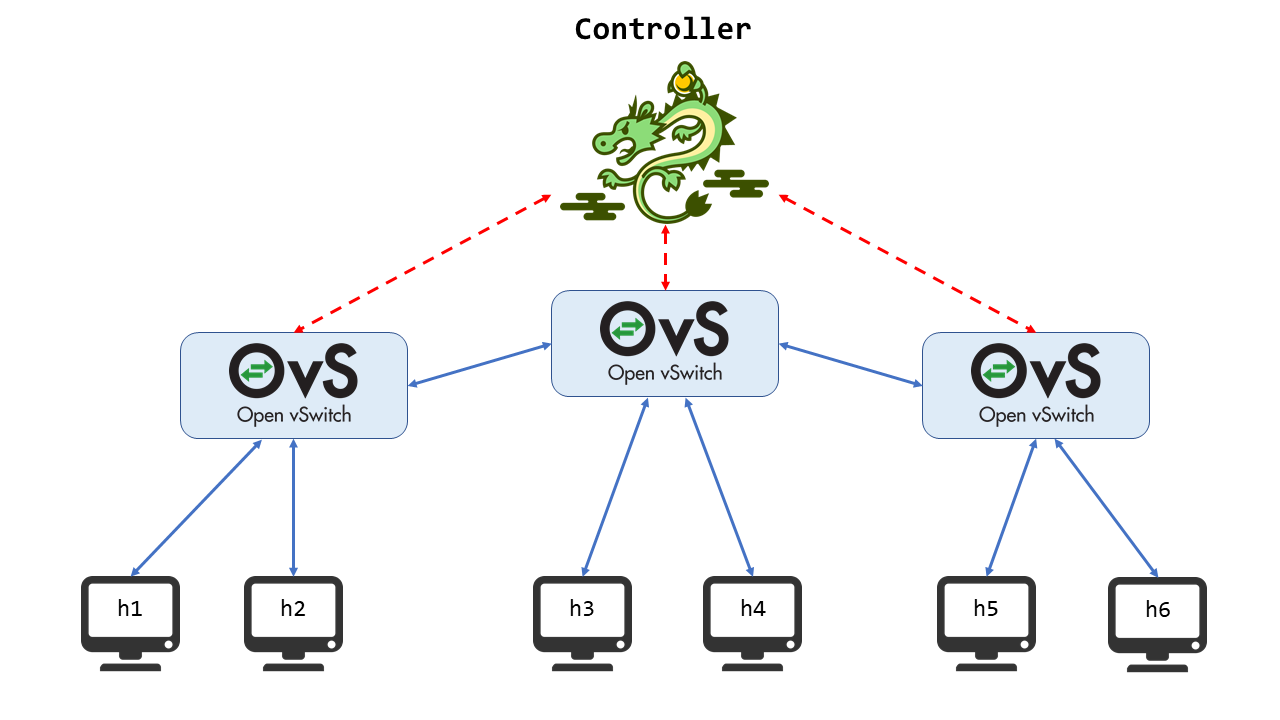
\includegraphics[width=\linewidth]{scenario.png}
		\caption{Mininet's Scenario}
		\label{f:scenario}
	\end{figure}

	Figure \ref{f:scenario} presents us with the \textit{logic} scenario we will be working with. As with many other areas in networking this logic picture doesn't correspond with the real implementation we are using. We have seen throughout the installation procedure how we are always talking about 2 VMs. If you read carefully you'll see that one VM's "names" are \textbf{controller} and \textbf{mininet}. So it should come as no surprise that the controller and the network itself are living in different machines!
	\newpar
	\newpar
	The first question that may arise is how on Earth can we logically join these 2 together. When working with virtualized environments we will generate a virtual LAN where each VM is able to communicate with one another. Once we stop thinking about programs and abstract the idea of "\textit{process}" we find that we can easily identify the \textbf{controller} which is just a \textbf{ryu} app, which is nothing more than a \textbf{python3} app with the \textbf{controller}'s VM \textbf{IP} address and the port number where the \textbf{ryu} is listening. We shouldn't forget that \textbf{any} process running within \textbf{any} host in the entire \textbf{Internet} can be identified with the host's \textbf{IP} address and the processes \textbf{port} number. Isn't it amazing?
	\newpar
	OK, the above sounds great but... Why should we let the controller live in a machine when we could have everything in a single machine and call it a day? We have our reasons:

	\begin{itemize}
		\item Facilitate teamwork, since the \textbf{AI's logic} will go directly into the controller's VM. This let's us increase both working group's independence. One may work on mininet's core and the data collection with \textbf{telegraf} whilst the other can look into the DDoS attack detection logic and visualization using \textbf{Grafana} and \textbf{InfluxDB}.
		\item Facilitate the storage of data into \textbf{InfluxDB} from \textbf{telegraf}, as due to the internal workings of Mininet there may be conflicts in the communication of said data. Mininet's basic operation at a low level is be detailed below.
		\item Having two different environments relying on distinct tools and implementing different functionalities let's us identify and debug problems way faster. We can know what piece of software is causing problems right away!
	\end{itemize}
    
    \subsection{Use case}
    Why this scenario and not another? That would be a question that would be asked by anyone who saw our project. Well, the fact that we have chosen this scenario and not another, is due to the benefits of Software Defined Networking (SDN). Among all the benefits we point out that it is possible to extract the control plane from the intermediate processing devices of the network, unifying it in entities called controllers, making the network administration a more centralized and flexible task.
    \newpar
    The detection system to be developed will benefit greatly from the fact that the control of the network is in a single machine, from which it will be possible to control or “instantiate” the rules necessary to mitigate the attacks previously detected by our system.
    \newpar
    So a practical application of our project can fit all the use cases of a SDN network. In our case we have chosen a small network with three switches. This is because we did not want to make the testing of our project too heavy, since we do not have very powerful machines to emulate a whole SDN core, it is going to be a “conceptual” sdn network. It is understood that the results obtained in this network are easily extrapolated to larger networks, because our project is not going to be very invasive with the SDN operation.
    \newpar
    If we want to particularize a little more in the case of use we can refer to the aggregation networks of an ISP (Internet service provider), which have the purpose of unifying different access networks of the clients. In this case, it is understood that the existence of an SDN in this aggregation network is reasonable, since as we have investigated it is usually a switch core. At the same time, we leave a figure \ref{f:usecase} that illustrates the concept of an aggregation network.
    
    \newpar
    
    In this way the ISP would have the capacity, thanks to our project, to detect if any of its clients is being victim of a DDoS attack, allowing it to mitigate it directly through the SDN controller.
    
    \newpage
    \begin{figure}[!htb]
			\centering
			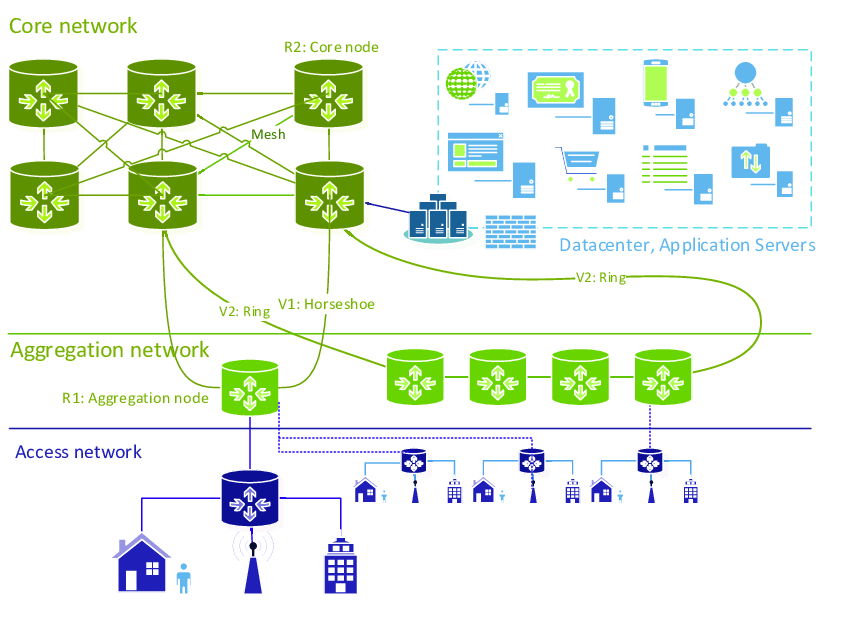
\includegraphics[width=\linewidth]{use_case.png}
			\caption{Aggregation network}
			\label{f:usecase}
	\end{figure}
	
	\subsection{Running the scenario}
		Running the scenario requires having logged into both VMs manually or using vagrant's SSH wrapper. First of all we're going to power up the controller, to do so we run the following from the \texttt{controller} VM. It's an application that does a basic forwarding, which is just what we need:

		\begin{minted}{bash}
	ryu-manager ryu.app.simple_switch_13
		\end{minted}

		You might prefer to run the controller in the background as it doesn't provide really meaningful information. In order to do so we'll run:

		\begin{minted}{bash}
	ryu-manager ryu.app.simple_switch_13 > /dev/null 2>&1 &
		\end{minted}

		Let's break this big boy down:

		\begin{itemize}
			\item \texttt{> /dev/null} redirects the \texttt{stdout} file descriptor to a file located in \texttt{/dev/null}. This is a "special" file in Linux systems that behaves pretty much like a black hole. Anything you write to it just "disappears". This way we get rid of all the bloat caused by the network startup.
			\item \texttt{2>\&1} will make the \texttt{stderr} file descriptor point where the \texttt{stdout} file descriptor is currently pointing (\texttt{/dev/null}). Terminal emulators usually have both \texttt{stdout} and \texttt{stderr}"going into" the terminal itself so we need to redirect these two to be sure we won't see any output.
			\item \texttt{\&} makes the process run in the background so that you'll be given a new prompt as soon as you run the command.
		\end{itemize}

		If you want to move the controller app back into the foreground so that you can kill it with \texttt{CTRL + C} you can run \texttt{fg} which will bring the last process sent to the background back to the foreground.

		\begin{figure}[!htb]
			\centering
			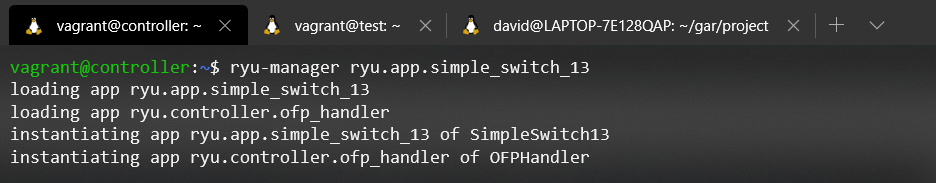
\includegraphics[width=\linewidth]{controller_ex.png}
			\caption{The controller is now running}
		\end{figure}

		Once the controller is up we are going to execute the network itself, to do so launch the aforementioned script from the \texttt{test} machine:

		\begin{minted}{bash}
	sudo python3 scenario_basic.py
		\end{minted}

        \newpage
		\begin{figure}[!htb]
			\centering
			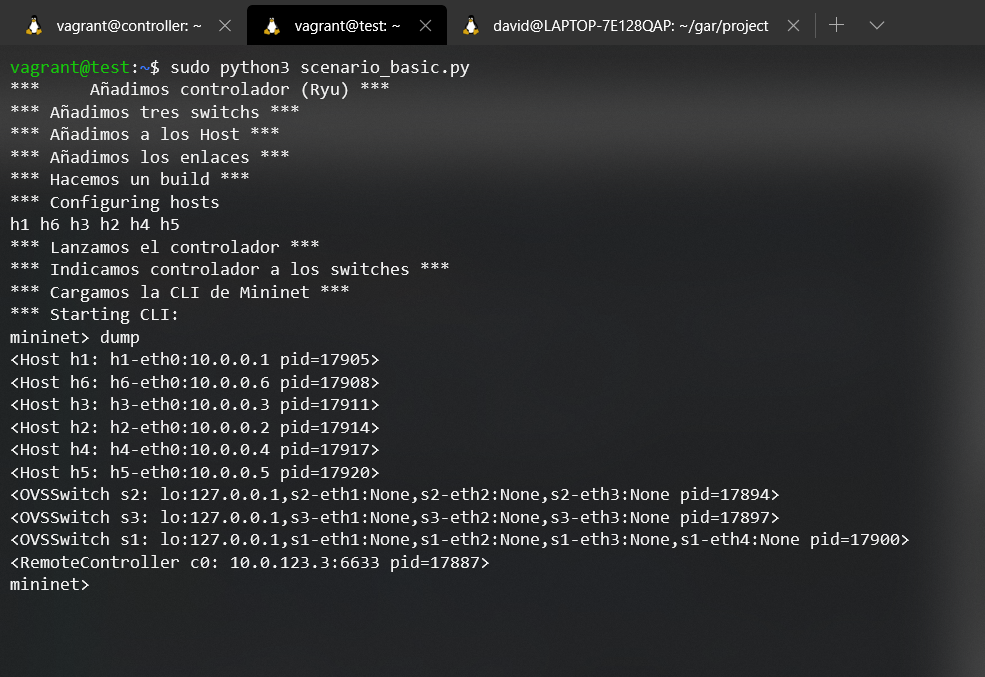
\includegraphics[width=\linewidth]{mininet_up.png}
			\caption{Mininet is now UP}
			\label{f:mininet_up}
		\end{figure}

		Notice how we have opened \textbf{Mininet CLI} from the \texttt{test} machine in figure \ref{f:mininet_up}. We can perform many actions from this command line interface. The most useful will be detailed below.

	\subsection{Is it working properly?}
		We should have our scenario working as intended by now. We can check our network connectivity by pinging the hosts, for example:

		\begin{minted}{bash}
	mininet> h1 ping h3

	# We can also ping each other with the pingall command
	mininet> pingall
		\end{minted}
        
        \newpage
		\begin{figure}
			\centering
			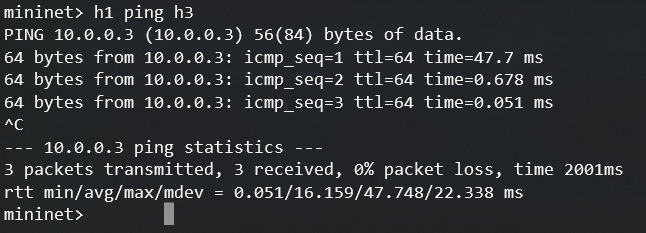
\includegraphics[width=\linewidth]{ping_ok.png}
			\caption{Mininet is working OK}
			\label{f:ping_ok}
		\end{figure}

		As you can see in figure \ref{f:ping_ok} there is full connectivity in our scenario. You may have noticed how the first  \textbf{ping} takes way longer than the other to get back to use. That is, its  \textbf{RTT} ( \textbf{R}ound  \textbf{T}rip  \textbf{T}ime) is abnormally high. This is due to the empty  \textbf{ARP} tables we currently have \textit{AND} to the fact that we don't yet have a flow defined to handle  \textbf{ICMP} traffic. We need to take a few steps to fix this:

		\begin{itemize}
			\item An \textbf{ARP} resolution between sender and receiver of the ping takes place so that the sender learns the next hop's \textbf{MAC} address.
			\item In addition, the \textbf{ICMP} message (ping-request) will be redirected to the driver (a.k.a controller) to decide what to do with the packet as the switches don't yet have a \textbf{flow} to handle this traffic type. This way the controller will, when it receives the packet, instantiate a set of rules on the switches so that the \textbf{ICMP} messages are routed from one host to the other.
		\end{itemize}
        \newpage
		\begin{figure}
			\centering
			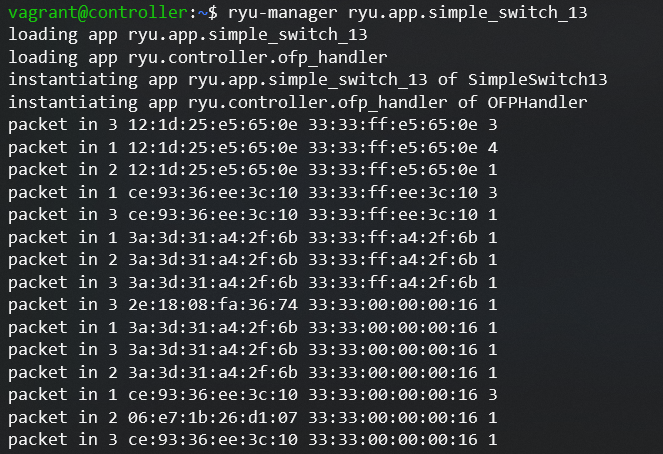
\includegraphics[width=\linewidth]{ryu_rcv.png}
			\caption{Ryu is configuring the flows}
			\label{f:ryu_rcv}
		\end{figure}

		As you can see in figure \ref{f:ryu_rcv}, the controller's \textbf{stdout} (please take a look at the appendix to learn more about file descriptors) indicates the commands it has been instantiating according to the packets it has processed. In the end, for the first packet we will have to tolerate a delay due to \textbf{ARP} resolution and \textbf{flow} lookup and instantiation within the controller. The good thing is the rest of the packets will already have the destination \textbf{MAC} and the rules will already instantiated in the intermediate switches, so the new delay will be minimal.

\newpage

\section{Attack Time}
	We have already talked about how to set up our scenario but we haven't got into breaking things (i.e the fun stuff  ). Our goal is to simulate a \textbf{DoS} (\textbf{D}enial \textbf{o}f \textbf{Service}) attack. Note that we usually refer to this kind of threats as \textbf{DDoS} attacks where the first \textbf{D} stands for \textbf{D}istributed. This second "name" implies that we have multiple machines trying to flood our own. We are going to launch the needed amounts of traffic from a single host so we would be making a mistake if we were talking about a distributed attack. All in all this is just a minor nitpick, the concept behind both attacks is exactly the same.
	\newpar
	We need to flood the network with traffic, great but... How should we do it? We already introduced the tool we are going to be using .
	\newpar
	The main objective is being able to classify the traffic in the network as a normal or an abnormal situation with the help of AI algorithms. For these algorithms to be effective we need some training samples so that they can "learn" how to regard and classify said traffic. That's why we need a second tool capable of generating "normal" ICMP traffic so that we have something to compare against. Good ol' \textbf{ping} is our pal here.

	\subsection{Time To Limit The Links}
		We should no mention our scenario again. We had a \textbf{Ryu} controller, three \textbf{OVS} switches and several hosts "hanging" from these switches. The question is: \textbf{what's the capacity of the network links?}
		\newpar
		According to Mininet's \href{https://github.com/mininet/mininet/wiki/Introduction-to-Mininet}{wiki} that capacity is not limited in the sense that the network will be able to handle as much traffic as the hardware emulating it can. This implies that the more powerful the machine, the larger the link capacity will be. This poses a problem to our experiment as we want it to be reproducible in any host. That's why we have decided to limit each link's bandwidth during the network setup.
		\newpar
		This behaviour is a consequence of Mininet's implementation. We'll discuss it when analyzing mininet's internals later on later down the road but the key aspect is that we cannot neglect Mininet's implementation when making design choices!

		\subsubsection{How To Limit Them}
			In order to limit the available \textbf{BW} (\textbf{B}and \textbf{W}idth) we'll use Mininet's API. This API is just a wrapper for a \textbf{TC} (\textbf{T}raffic \textbf{C}ontroller) who is in charge of modifying the kernel's \textbf{planner} (i.e \textit{Network Scheduler}). The code where we leverage the above is:

			\begin{minted}{python}
	net = Mininet(topo = None,
				build = False,
				host = CPULimitedHost,
				link = TCLink,
				ipBase = '10.0.0.0/8')
			\end{minted}

			Note how we need to limit each host's capacity by means of the CPU which is what we do through the \texttt{host} parameter in Mininet's constructor. We'll also need links with a \texttt{TCLink} type. We can achieve this thanks to the \texttt{link} parameter. This will let us impose the limits to the network capacity ourselves instead of depending on the host's machines capabilities.
			\newpar
			After fiddling with the overall constructor we also need to take care when defining the network links. We can find the following lines over at \textbf{src/scenario\_basic.py}:

			\begin{minted}{python}
	net.addLink(s1, h1, bw = 10)
	net.addLink(s1, h2, bw = 10)
	net.addLink(s1, s2, bw = 5, max_queue_size = 500)
	net.addLink(s3, s2, bw = 5, max_queue_size = 500)
	net.addLink(s2, h3, bw = 10)
	net.addLink(s2, h4, bw = 10)
	net.addLink(s3, h5, bw = 10)
	net.addLink(s3, h6, bw = 10)
			\end{minted}

			We are fixing a \textbf{BW} for the links with the \texttt{bw} parameter. We have also chosen to assign a finite buffer size to the middle switches in an effort to get as close to reality as we possibly can. If the \texttt{max\_queue\_size} parameter hadn't been defined we would be working with "infinite" buffers at each switch's exit ports. Having these finite buffers will in fact introduce a damping effect in our tests as once you fill them up you can't push any more data through: the output queues are absolutely full... In a real-life scenario we would suffer huge packet losses at the switches and that could be used as a symptom as well but we haven't taken it into account for the sake of simplicity.\newline
			\newline
			We fixed the queue lengths so that they were coherent with standard values. We decided to use a \textbf{500 packet} size because \textit{Cisco}'s queue lengths range from 64 packets to about 1000 as found \href{https://www.cisco.com/c/en/us/support/docs/routers/7200-series-routers/110850-queue-limit-output-drops-ios.html}{here}. We felt like 500 was an appropriate value in the middle ground. With all these restrictions our scenario would look like figure \ref{f:limited}.
            
    
			\begin{figure}[!htb]
				\centering
				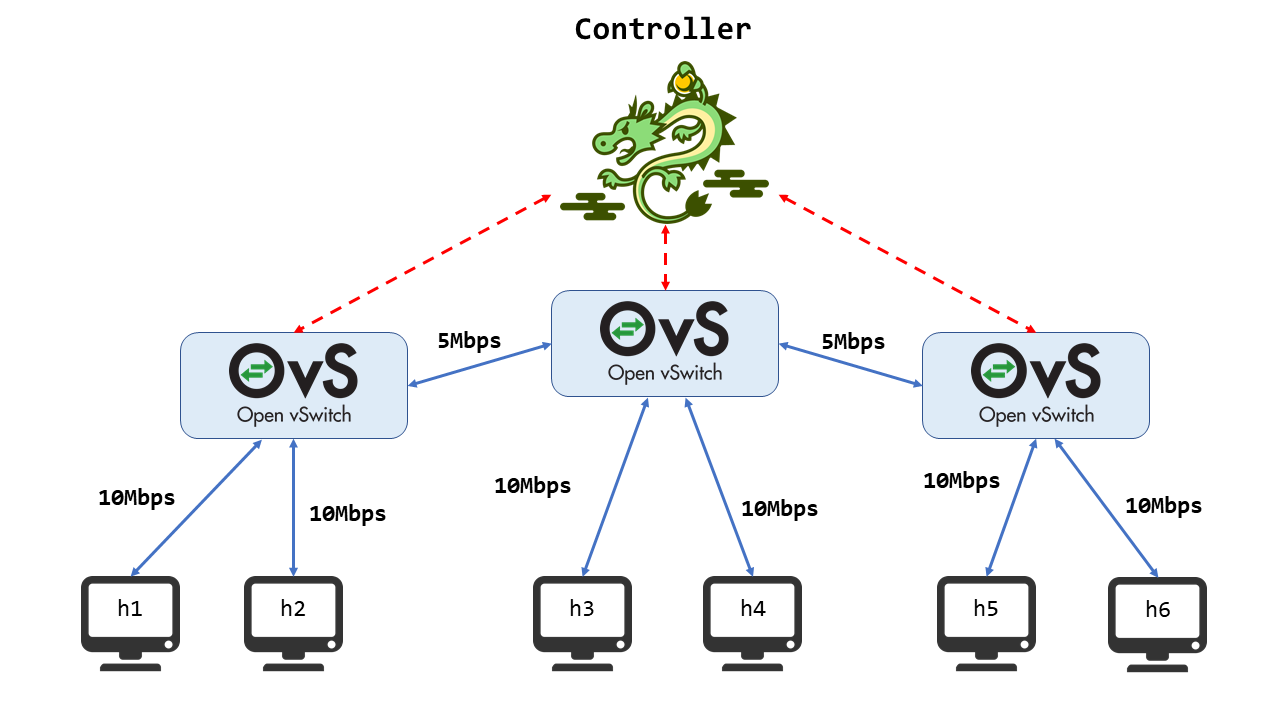
\includegraphics[width=\linewidth]{scenario_limits.png}
				\caption{Scenario with link capacities}
				\label{f:limited}
			\end{figure}

			By inspecting the network dimensions we can see how we have a clear bottleneck... This "flaw" has been introduced on purpose as we want to clearly differentiate regular traffic from the one we experience when under attack.

	\subsection{Getting Used to \texttt{hping3}}
		This versatile tool can be configured so that it can explore a given network, perform traceroutes, send pings or carry out out flood attacks on different network layers. All in all, it lets us craft our own packets and send them to different destinations at some given rates. You can even forge the source \textbf{IP} address to go full stealth mode   \textbf{ICMP --> Echo request (Type = 8, Code = 0)} whilst increasing the rate at which we send them. This will in turn make the network core collapse making our attack successful.
		\newpar
		Check out this \href{https://tools.kali.org/information-gathering/hping3}{site} for more info on this awesome tool.

	\subsection{Installing Things... Again!}
		The tool will be already present on the test machine as it was included in the \textbf{Vagrantfile} as part of the VM's provisioning script. In case you want to manually install it you can just run the command below as \textbf{hping3} is usually within the default software sources:

		\begin{minted}{bash}
	sudo apt install hping3
		\end{minted}

	\subsection{Usage}
		As we have previously discussed this is quite a complete tool so we will only use one of the many functionalities to keep things simple. The command we'll be using is:

		\begin{minted}{bash}
	hping3 -V -1 -d 1400 --faster <Dest_IP>
		\end{minted}

		We are going to break down each of the options:

		\begin{itemize}
			\item \texttt{-V}: Show verbose output (i.e show more information)
			\item \texttt{-1}: Generate ICMP packets. They'll be ping requests by default
			\item \texttt{-d 1400}: Add a bogus payload. This is not strictly needed but it'll help us use up the link's BW faster. We have chosen a 1400 B payload so as not to suffer fragmentation at the network layer.
			\item \texttt{--faster}: If we used the \texttt{flood} option we overwhelmed the virtualized network...
		\end{itemize}

		We would like to point out that \texttt{hping3} could have been invoked with the \texttt{--flood} option instead of \texttt{--faster}. When using \texttt{--flood} the machine will generate as many packets as it possibly can. This would be great in a world of rainbows but... The virtual network was quickly overwhelmed by the ICMP messages and packets began to be discarded everywhere. Event though this is technically a \textbf{DoS} attack gone right too it obscures the phenomena we are faster so we decided to use \texttt{--faster} as the rate it provides suffices for our needs.

	\subsection{Demo Time!}
		The attack we are going to carry out comprises hosts \textbf{1}, \textbf{2} and \textbf{4}. We'll launch \texttt{hping3} from \textbf{Host1} targeting \textbf{Host4} and we'll try to ping \textbf{Host4} from \textbf{Host2}. We will in fact see how this "regular" ping doesn't get through as a consequence of a successful \textbf{DoS} attack. Figure \ref{f:dos_atk} depicts the situation.

		\begin{figure}[!htb]
			\centering
			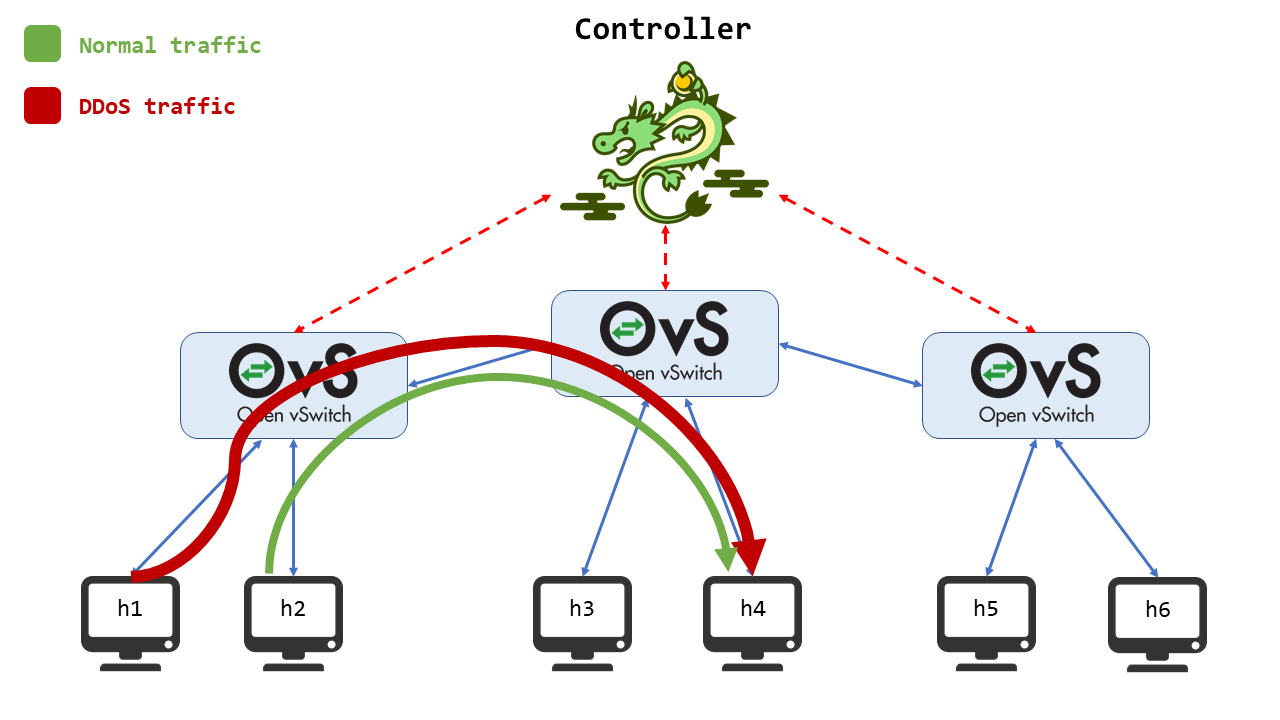
\includegraphics[width=\linewidth]{scenario_ddos.png}
			\caption{Under attack!}
			\label{f:dos_atk}
		\end{figure}
        
        \newpage
		Let's begin by setting up the scenario like we usually do:

		\begin{minted}{bash}
	sudo python3 scenario_basic.py
		\end{minted}

		Time to open terminals to both ICMP sources. We'll also fire up \texttt{Wireshark} on \textbf{Host4} to have a closer look at what's going on. Note the ampersand (\texttt{\&}) at the end of the second command. It'll detach the \texttt{wireshark} process from the terminal so that we can continue running commands as we normally would. To do this we need to run:

		\begin{minted}{bash}
	mininet> xterm h1 h2
	mininet> h4 wireshark &
		\end{minted}


        Time to launch \texttt{hping3} from \textbf{Host1} with the parameters we discussed. This is shown in figure \ref{f:hping3_ex}.
		\begin{figure}[!htb]
			\centering
			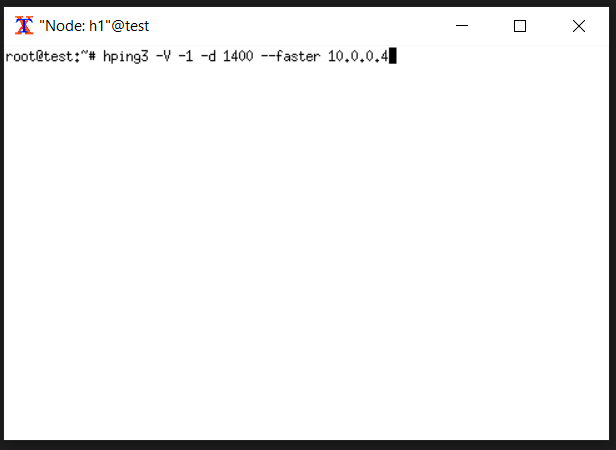
\includegraphics[width=\linewidth]{launch_hping3.png}
			\caption{Launching the \texttt{DoS} attack}
			\label{f:hping3_ex}
		\end{figure}

        \newpage		
		If we now try to ping \textbf{Host4} from \textbf{Host2} we'll fail horribly as we find in figure \ref{f:net_down}.

		\begin{figure}[!htb]
			\centering
			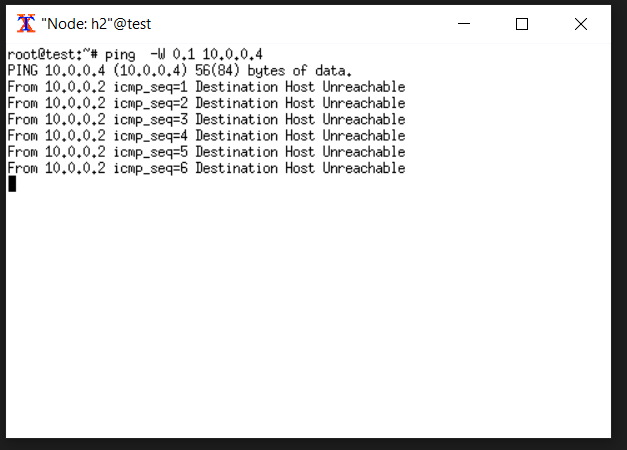
\includegraphics[width=\linewidth]{net_down.png}
			\caption{\texttt{ICMP} traffic can't get through...}
			\label{f:net_down}
		\end{figure}

		If we halt the \textbf{DoS} attack we will see the regular traffic resume its normal operation after a short period of time. Figure \ref{f:net_ok} depicts this.
		\newpar

		\begin{figure}[!htb]
			\centering
			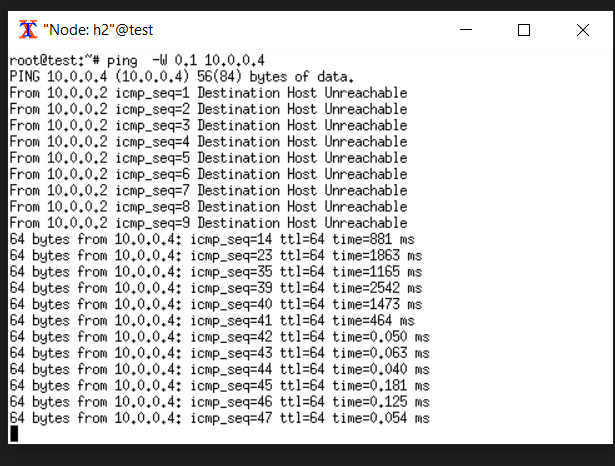
\includegraphics[width=\linewidth]{net_ok.png}
			\caption{The network has recovered!}
			\label{f:net_ok}
		\end{figure}

		We then see how the \textbf{DoS} attack against \textbf{Host4} has been successful. In order to facilitate issuing the needed commands we have prepared a couple of \texttt{python} scripts containing all the needed information so that we only need to run them and be happy. You can find them at:

		\begin{itemize}
			\item Attack \href{https://github.com/GAR-Project/project/blob/master/src/ddos.py}{\texttt{src/ddos.py}}
			\item Regular traffic \href{https://github.com/GAR-Project/project/blob/master/src/normal.py}{\texttt{src/normal.py}}
		\end{itemize}

		With all this ready to rock we now need to focus on detecting these attacks and seeing how to possibly mitigate them.

	\subsection{Wanted a Video}
		You can find a video showing the process we described step by step \href{https://www.youtube.com/watch?v=ofZPmV6_y_M}{here}. If you stumble upon any questions don't hesitate to contact us!

\newpage

\section{Traffic Classification With a SVM (\textbf{S}upport \textbf{V}ector \textbf{M}achine)}
	We have our scenario working properly and the attack is having the desired effect on our network. In other words, it's blowing things up. If we are to detect the attack we need to gather representative data and process it somehow so that we can predict whether we are under attack or not. As Jack the Ripper once said, let's break this into parts. We'll begin by gathering the necessary data and sending it to a database we can easily query. We'll then prepare training datasets for our SVM and get it ready for making guesses. Let's begin!

	\subsection{First Step: Getting The Data Collection To Work}
		\subsubsection{What Tools Are We Going To Use?}
			For a previous project belonging to the same subject we were introduced to both \textbf{telegraf} and \textbf{influxdb}. The first one is a metrics agent in charge of collecting data about the host it's running on. It's entirely plug-in driven so configuring it is quite a breeze! The latter is a \textbf{DBMS} (\textbf{D}ata\textbf{B}ase \textbf{M}anagement \textbf{S}ystem) whose architecture is specifically geared towards time series, just what we need! The interconnection between the two is straightforward as one of \textbf{telegraf}'s plug-ins provides native support for \textbf{influxdb}. We'll have to configure both appropriately and we'll see it wasn't as easy as we once thought due to mininet getting in the way. We have come up both with a "hacky" solution and an alternative any Telecommunications Engineer would be prod of. Just kidding, but it uses networking concepts and not workarounds though.

		\subsubsection{Leveraging Mininet's Shared Filesystem}
			Have you ever felt like throwing yourself into \texttt{/dev/null} to never come back? That was pretty much our mood when trying to get a host within mininet's network to communicate with the outside world. In order to understand how we ended up "fixing" (it just works  ) everything we need to go back and take a look at our initial ideas and implementations.
			\newpar
			We should not forget that we are looking at \texttt{ICMP} traffic in order to make predictions about the state of the network. We first thought about running \textbf{telegraf} on a network switch that was directly connected to the controller where our \textbf{InfluxDB} instance is running. The good thing about this scheme is that the telegraf process within the switches can communicate with the DB running in the controller through \texttt{HTTP}. This is due to the fact that we are invoking the \texttt{start()} method of the switches during the network configuration so even though there's no "real" link between them (we didn't create it by calling \texttt{addLink()}) they can still communicate.
			\newpar
			The above sounds wonderfully well but... switches can only work with information up to the \textbf{link layer}, they know nothing about \textbf{IP} packets or \textbf{ICMP} messages. We should note that \textbf{ICMP} is a layer 3-ish (more like layer 3.5) protocol. As it relies on IP for the network services but doesn't have a port number we cannot assign a particular layer to it... All in all the switches knew nothing about ICMP messages crossing them so we find that we need to run telegraf on one of the hosts if we want to get our metrics. In a real case scenario we could devote a router (which can process ICMP data) instead of a switch for this purpose and reconfigure the network accordingly. Anyway we need to get the telegraf instance running in one of the mininet created hosts to communicate with the influx database found in the controller VM. Let's see how we can go about it...
			\newpar
			When discussing the internal mechanisms used by mininet later on we'll find out that it relies solely on network namespaces. This implies that the filesystem is shared across the network elements we create with mininet \textbf{AND} the host machine itself. This host machine has direct connectivity with the VM hosting the controller so we can take advantage of what others consider to be a flaw in mininet's architecture. We are going to run a telegraf instance on mininet's \texttt{Host 4} whose input plug-in will gather ICMP data and whose output will be a file in the VM's home directory. We'll be running a second telegraf instance in the host VM whose input will be the file containing \texttt{Host 4}'s output and whose output will be the Influx DB hosted in the controller VM. This architecture leverages the shared filesystem and uses a second telegraf instance as a mere proxy between one of mininet's internal hosts and the controller VM, both living in entirely different networks.
			\newpar
			In order to implement this idea we have created all the necessary configuration files under \texttt{conf} to then copy them to the appropriate places during Vagrant's provisioning stage.

		\subsubsection{Implementing A NAT (\textbf{N}etwork \textbf{A}ddress \textbf{T}ranslator) In Mininet For External Communication}
			Once we implemented the solution above we were able to continue developing the \textbf{SVM} as we already had a way of retrieving data. That's why we decided to devote some time to looking for a more elegant solution. Just like we usually do in home LANs we decided to instantiate a NAT process to get interconnection to the network created for the VM's from within the emulated one. Due to problems with the internal functioning of this NAT process provided by Mininet, extra configuration had to be added to achieve the desired connectivity. To solve the problem a series of predefined rules (flows) were installed in each switch to "route" the traffic from our data collector to the NAT process and from there to the outside to InfluxDB.  This could be considered a "fix", but in fairness we are only using the logic of an SDN network to route our traffic in the desired way.  You can take a closer look at this implementation \href{https://github.com/GAR-Project/project/tree/full-connectivity}{in this branch}.

		\subsubsection{What Data Are We Going To Use?}
			We are trying to overwhelm \texttt{Host 4} with a bunch (a \textbf{VERY BIG} bunch) of \texttt{ICMP Echo Requests} (that is fancy for \texttt{pings}). By reading through telegraf's input plug-in list we came across the \textbf{net} plug-in capable of providing \texttt{ICMP} data out of the box.

		\subsubsection{Getting The Data To \texttt{InfluxDB}}
			Instead of directly sending the output to an influxdb instance we are going to send it to a regular file thanks to the \textbf{file} output plug-in. This leads us directly to the configuration of the second telegraf instance.
			\newpar
			In this second process we'll be using the \textbf{tail} input plug-in. Just like Linux's \texttt{tail}, this command will continuously read a file so that it can use it as an input data stream. Instead of polling the file continuously we chose to instead notify telegraf to read it when changes took place. This leads to a more efficient use of system resources overall. The output plug-in we'll be using is now good ol' \textbf{influxdb}. We'll point it to the influxdb instance running on the \texttt{controller} VM so that everything is correctly connected.
			\newpar
			The structure of the system we are dealing with is shown in figure \ref{f:telegraf_connections}.

			\begin{figure}
				\centering
				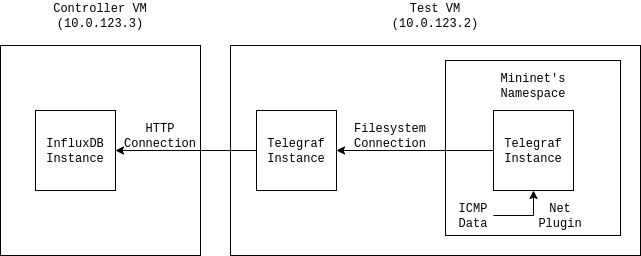
\includegraphics[width=\linewidth]{telegraf_connections.png}
				\caption{Connection through the filesystem}
				\label{f:telegraf_connections}
			\end{figure}

			We are now ready to start querying our database and begin working with the acquired information.

		\subsubsection{A Note On The Sampling Period}
			When configuring the interconnection between both telegraf instances we initially left the default \texttt{10 s} refresh interval in both. When we read the data we were getting in the DB we noticed some "strange" results in between correct readings so we decided to fiddle with these sampling times in case they were interfering with each other. As we are communicating both processes by means of a file the timing for reading and writing can be critical... We fixed a \texttt{2 s} sampling interval in "mininet's" telegraf process and a \texttt{4 s} refresh rate in the VM's instance. This means that we are going to get 2 entries in the DB with each update!
			\newpar
			After running some tests we found everything was working flawlessly now   so we just left it as is.

	\subsection{Second Step: Generating the Training Datasets}
		\subsubsection{Weren't we using the received \texttt{ICMP} messages as the input?}
			Well... yes and no. The cornerstone for the SVM's input is indeed the number of received ICMP messages \textbf{BUT} we decided to use the \textit{derivative} of the incoming packets with respect to time instead of the absolute value. This approach will let the network admin apply the exact same SVM for attack detection even if the traffic increases due to a network enlargement. As we are looking for sudden changes in incoming messages rather than for large numbers this approach is more versatile.
			\newpar
			After debating it for a while we settled on including the average of the derivative of the incoming packets as a parameter too. As the mean will vary slowly due to the disparity of the data generated by both situations we'll be more likely to consider the aftermath as an attack too. Even though we may not be subject to very high incoming packet variations any more we'll take a while to resume a normal operation and we decided to let this "recovery time" play a role in the SVM's prediction.

		\subsubsection{Writting a Script: \texttt{src/data\_gathering.py}}
			Once we have the desired data stored in the DB using the SVM becomes a matter of reading it and formatting it so that the SVM "likes it". In order to make the process faster we decided to write a simple python script that uses influxdb's python API to read the data and prepare a \textbf{CSV} (\textbf{C}omma \textbf{S}eparated \textbf{V}alues) to later be read by the script implementing the SVM.
			\newpar
			The defining quality of training data is meaningfulness. The SVM's predictions will only be as good as the training it received so we need to provide insightful data if we are to get any consistent results.
			\newpar
			In order to get appropriate data samples we went ahead an simulated regular traffic by pinging the target host at a rate of roughly 1 ICMP message per second. We then attacked the target until we got around 100 samples into de DB.
			\newpar
			Generating the DB is just a matter of reading the DB and outputting the read data to a text file with a \texttt{.csv} extension.

	\subsection{Third Step: Putting it all together}
		Before analyzing \texttt{traffic\_classifier.py} let's do a little bit of...

		\subsubsection{A Tiny Bit of Math}
			As one of the parameters we feed the \textbf{SVM} is the mean of the data we get from the terminal we tried to come up with an scalable way of computing it as more samples came instead of recomputing the mean taking all the values into acount. This naive approach would have needed an ever growing array to store all the data, meaning it would have eventually exhausted the machine's resources... By taking a look at the estimator for the mean ($\hat{x}$) we tried to compute $\Delta\hat{x}$ by taking its previous values into account. Working with the equations yielded:

			\begin{equation}
				\label{eq1}
				\begin{split}
					\hat{x}_f & = \hat{x}_o + \Delta\hat{x} \rightarrow \Delta\hat{x} = \hat{x}_f - \hat{x}_o = \\
							  & = \frac{\alpha + \omega}{\beta + 1} - \frac{\alpha}{\beta} = \\
							  & = \frac{\beta(\alpha + \omega) - \alpha(\beta + 1)}{\beta(\beta + 1)} = \\
							  & = \frac{\alpha + \omega - \hat{x}_o\beta - \hat{x}_o}{\beta + 1} = \\
							  & = \frac{\omega - \hat{x}_o}{\beta + 1} \rightarrow \\
							  & \rightarrow \Delta\hat{x} = \frac{\omega - \hat{x}_o}{\beta + 1}
				\end{split}
			\end{equation}

			As seen in \ref{eq1} all we need to do is compute the new mean as $\hat{x}_f = \hat{x}_o + \Delta\hat{x}$ and to compute $\Delta\hat{x}$ we only need the previous mean ($\hat{x}_o$) and values $\omega,\ \beta$ which are the incoming sample's value and the previous number of samples respectively. This let's us continue to compute the mean indefinitely as long as we store the previous mean and number of recorded samples. You can find this procedure in the \texttt{work\_time()} method within the \texttt{src/traffic\_classifier.py} script.

		\subsubsection{Writing the Script}
			Apart from the scenario's setup the most important program we wrote is the \texttt{traffic\_classifier} without a doubt. The file defines the \texttt{gar\_py()} class which includes a SVM instance, the query used for getting data and many other configuration parameters as its attributes. This let's us use this same technique in other scenarios, in other words, we are increasing this solution's portability.
			\newpar
			The class' constructor will limit itself to initializing its attributes and training the SVM by reading the training files we have already prepared. The main thing to note here is how we need to conform to the input format accepted by the SVM itself.
			\newpar
			Once it's trained we just need to call the class's \texttt{work\_time()} method which will enter an infinite loop whose operation can be summarised into these points:

			\begin{enumerate}
				\item Read the last 3 entries in the DB.
				\item Verify these entries are indeed new.
				\item Update the parameters we're going to use for the prediction.
				\item Order the SVM to predict whether the new data represents an attack or not.
				\item Write an entry to the appropriate DB signalling whether or not we're under attack.
				\item Wait 5 seconds to read new data. New data is sent to the DB every 4 seconds so reading insanely fast is just throwing resources out the window.
			\end{enumerate}

			Additionally we used \texttt{matplotlib} to draw the classification we were carrying out. As you can see in figure \ref{f:svm_graph}, the red dots are those data that have been classified as an anomalous traffic, DDoS traffic, and although it seems that there is only one blue dot belonging to "normal" traffic, it is not the case, there are several but their deviation between them is minimal.

			\begin{figure}
				\centering
				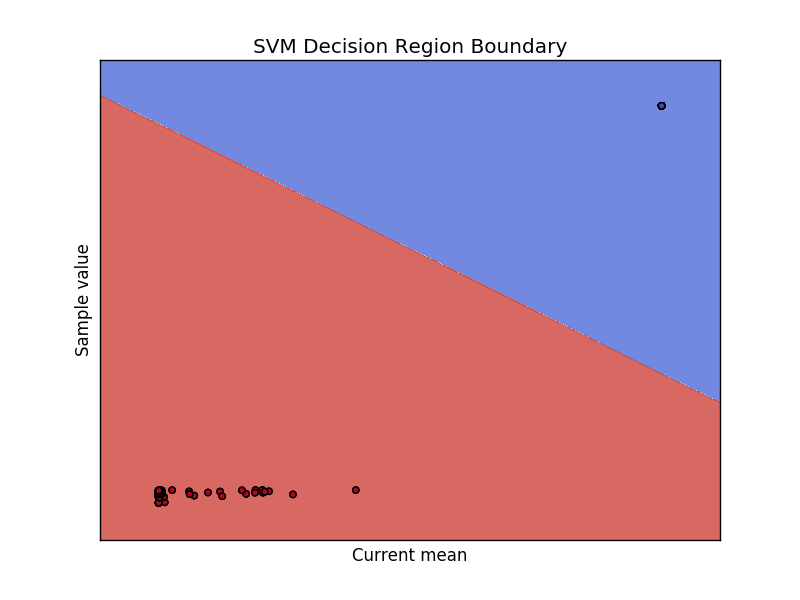
\includegraphics[width=\linewidth]{svm_graph.png}
				\caption{SVM's Decision Regions}
				\label{f:svm_graph}
			\end{figure}

			We've also written a signal handler to allow for a graceful exit when pressing \texttt{CTRL + C}.
			\newpar
			And with that we are finished! We hope to have been clear enough but if you still have any questions don't hesitate to contact us. You can find our GitHub at the end of the document.

\newpage

\section{Net Status Visualization with the \texttt{Grafana} + \texttt{InfluxDB} + \texttt{Telegraf} tool set}
	We have already discussed how to retrieve significant data from the hosts within mininet's network. The thing is this gathered data is nothing more than a collection of numbers whose interpretation can be quite tricky if we don't have a very clear idea of the system we are dealing with. We have seen how the traffic classifier's output was a new measurement within the \texttt{h4\_net\_stats} database within \texttt{InfluxDB}. We also talked about the process that let us "sneak" the data past mininet's own network so we are left with the task to interconnect \texttt{grafana} and \texttt{influxdb} so that we can get the visualization going. Even though we have already stated it, we feel like we should inform the reader that the installation of all these programs is handled by \texttt{vagrant}'s provisioning scripts: everything from the download of the correct binaries to the management of the associated service files with \texttt{systemd} has been taken care of.
	\newpar
	we'll begin by digging a little bit deeper into \texttt{grafana} as it's the tool we have described the least. We'll then briefly go through \texttt{influxdb}'s and \texttt{telegraf}'s data gathering configuration as well. We are doing this for completeness' sake, we should stress once more that the end user doesn't need to deal with.

	\subsection{Configuring \texttt{Grafana}}
		Grafana is a visualization platform. This implies that \texttt{grafana} itself \textbf{doesn't} gather any data and it \textbf{won't} store it either. This is where \texttt{telegraf} and \texttt{influxdb} come into play respectively. Having such a modular design allows for changes in the way we gather or store the data whilst maintaining the same monitoring interface. Now, we need to figure out how to get all these three services working cohesively and that's where configuration comes into play. We can take a look at the system we need to handle in figure \ref{f:g_i_t}.

		\begin{figure}
			\centering
			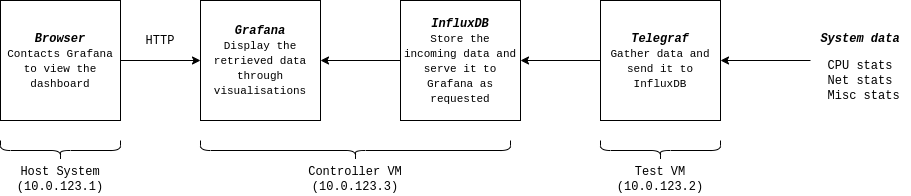
\includegraphics[width=\linewidth]{g_i_t.png}
			\caption{\texttt{Grafana}'s, \texttt{Influx}'s and \texttt{Telegraf}'s connections scheme}
			\label{f:g_i_t}
		\end{figure}

		The configuration limits itself mostly to editing files under the \texttt{/etc} directory in the VMs. Let's dive into \texttt{grafana}'s and \texttt{influxdb}'s interconnection.

		\subsubsection{Feeding data to \texttt{Grafana}}
			\texttt{Grafana} and \texttt{influxdb} will communicate through \texttt{HTTP} messages. That's why the only "thing" we need to tell \texttt{grafana} to reach the database whose data we are interested in is the \texttt{IP:port} tuple identifying the machine hosting \texttt{inluxdb} and the port it's listening on. As we are running \texttt{grafana} in the same machine as the database and we are using \texttt{influx}'s default port we just need to use \textbf{\texttt{http://localhost:8086}} to reach \texttt{influxdb}. We now need to specify the database we want to query. As we have previously discussed we need to take a look at the \texttt{h4\_net\_stats} DB so we'll go ahead and configure that as well.
			\newpar
			The above process can be either carried out manually with \texttt{grafana}'s GUI or we can opt to provide a \texttt{.yml} provisioning file to be used when starting up the service to configure the data sources in a headless way. We opted to g this route to facilitate the deployment of the scenario. You can find the data source configuration files over at \texttt{conf/datasources.yaml} in the GitHub repository. This file must be located at \texttt{/etc/grafana/provisioning/datasources} in the machine running \texttt{grafana}.

		\subsubsection{Hacker mode on: Preparing the Dashboard}
			We now have a way of getting data into \texttt{grafana} but we haven't provided any way of visualizing it... That's where the dashboard comes in. We'll use \texttt{grafana}'s GUI to prepare a set of visualizations ranging from bar graphs to doughnut meters to try and find a coherent and efficient way of determining the network state at a glance. In order to make the dashboard more visually appealing we are also showing measurements related to other aspects of the network, not only those regarding the \texttt{DoS} attack detection. In order to get these measurements we had to tinker with telegraf's configuration. We'll get into it below. You can find a picture portraying our super cool dashboard in figure \ref{f:dashboard}.

			\begin{figure}
				\centering
				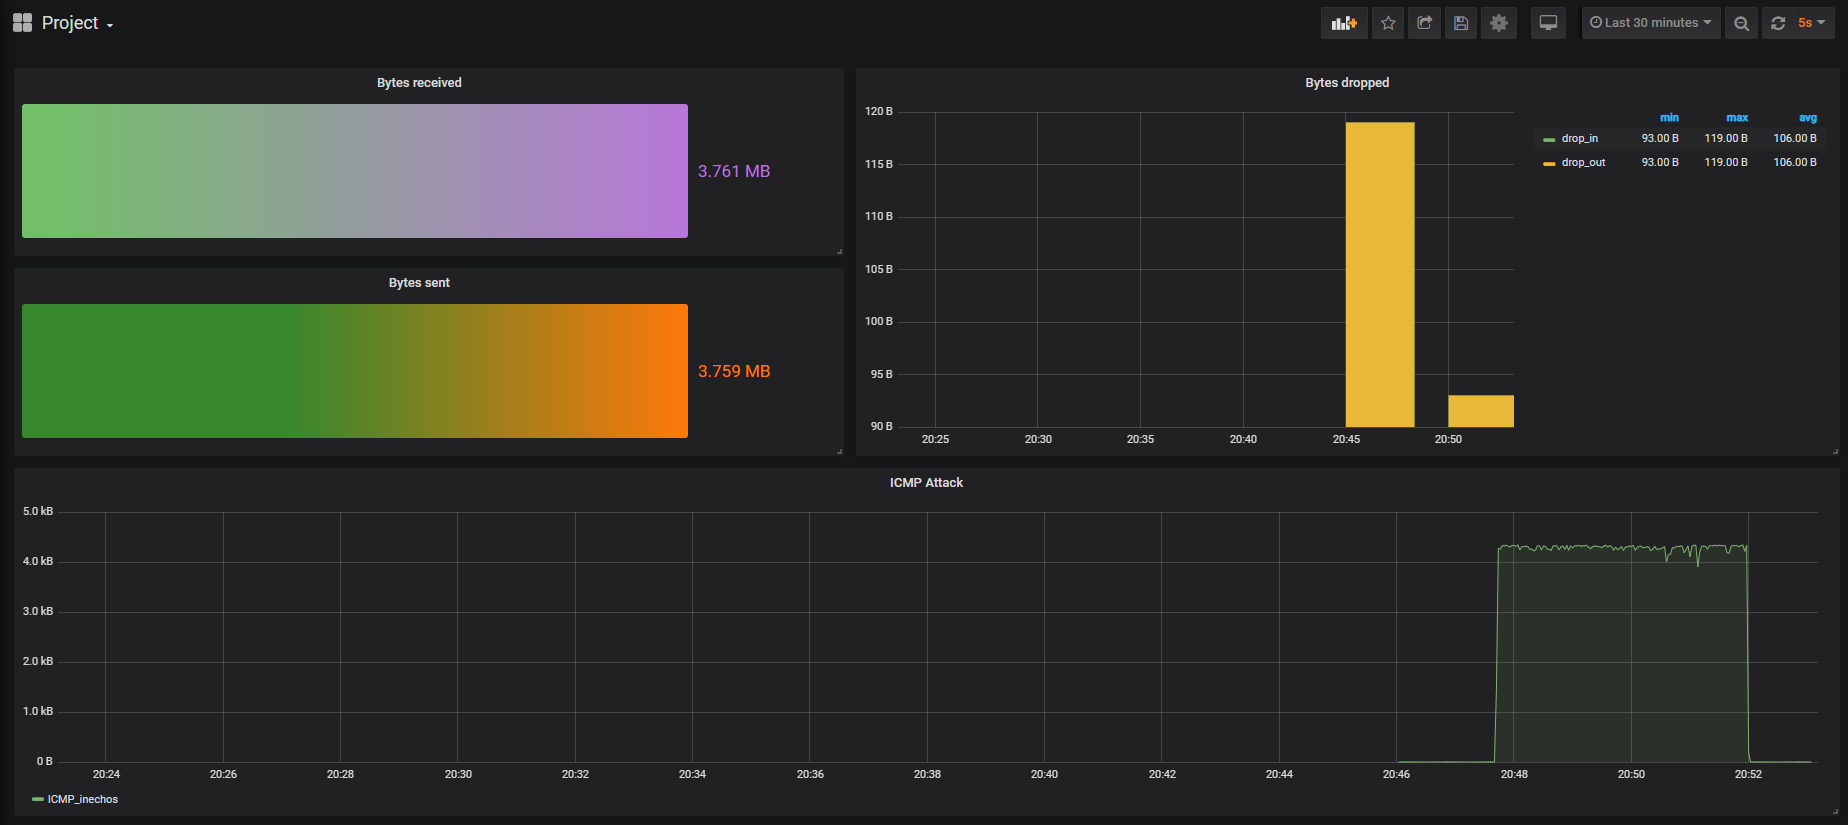
\includegraphics[width=\linewidth]{dashboard.png}
				\caption{\texttt{Grafana}'s dashboard}
				\label{f:dashboard}
			\end{figure}

			In order to facilitate sharing and reinstalling dashboards \texttt{grafana} has a handy export functionality that let's us save our dashboards as \texttt{JSON} (\textbf{J}ava\textbf{S}cript \textbf{O}bject \textbf{N}otation) files. These can be seamlessly provisioned to \texttt{grafana} just like we did with the data source configuration before. You can find the file handling this process over at \texttt{conf/main.yaml} which needs to be located at \texttt{/etc/grafana/provisioning/dashboards}. The dashboard itself is located at \texttt{conf/project\_dashboard.json}. This file needs to be located at \texttt{/var/lib/grafana/dashboards} so that our provisioning file can find it!
			\newpar
			We are now ready to delve deeper into the configuration regarding the database in charge of storing all this data. Enter \texttt{InfluxDB}.

	\subsection{Configuring  \texttt{InfluxDB}}
		Getting \texttt{influxdb} to work is actually quite a breeze. We can just use the default configuration and take it into account when configuring the other tools. As you might have guessed, \texttt{influxdb} exposes a \texttt{HTTP} entry point on port \texttt{8086} which is what we used when configuring \texttt{grafana} above. You can run \texttt{influx} on a shell within the \texttt{controller} VM to check that everything is working correctly. The command will open a DB management system where we can select what DB to query and perform operations on. As we haven't started \texttt{telegraf} yet we'll see no database has been created... yet. You can find a screenshot showing \texttt{influx}'s management system in figure \ref{f:influx}.

		\begin{figure}
			\centering
			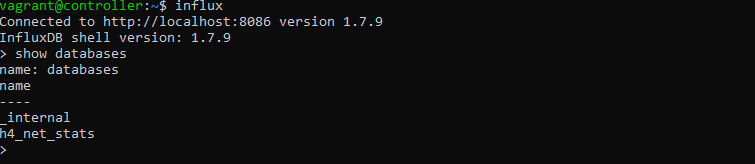
\includegraphics[width=\linewidth]{influx.png}
			\caption{\texttt{Influx}'s management system}
			\label{f:influx}
		\end{figure}

	\subsection{The last piece of the puzzle: \texttt{telegraf}}
		\texttt{Telegraf}'s configuration is carried out through \texttt{.conf} files under \texttt{/etc/telegraf} in each machine we want to gather data from. We have already explained the logic behind the filesystem bypass we implemented to "escape" mininet's cage. What we didn't do however is getting into how the "trick" was implemented. In order to get a high level overview of how \texttt{telegraf} works we need to talk about \texttt{plugins}:
		\newpar
		\texttt{Telegraf} is characterized by the implicit modularity of its design. All the data it gathers comes through \texttt{input plugins} and all the data it relays or outputs passes through its \texttt{output plugins}. We should point out that there are a few "gloabal" configuration parameters for the \texttt{telegraf} agent itself; the defaults are acceptable so we can focus solely on the \texttt{I/O} plugins. Following this approach we find how we only need to configure an output plugin to send \texttt{telegraf}'s output to \texttt{influxdb} and we need to choose the appropriate input plugins to gather data of interest for our project. We chose to use the \texttt{net} input plugin to access \texttt{ICMP} data but there are loads of plugins for gathering from  the current memory usage to the total process count in the monitored system. Taking this into account let's us tinker with \texttt{telegraf} in a pretty easy and intuitive way whilst abstracting ourselves from the \texttt{OS} running "under" us.
		\newpar
		Now, as \texttt{influxdb}'s \texttt{API} is web based we only need to provide the address of the machine hosting it (\texttt{localhost} in our case) and we'll be ready to rock. We'll notice how a \texttt{telegraf} database will be created seconds after starting \texttt{telegraf}'s service. All the data we'll gather is contained within this DB so we only need to configure \texttt{grafana}'s dashboard to query it and \textbf{magic}, it just works! You can find a screenshot portraying the status of the \texttt{telegraf} daemon over at figure \ref{f:telegrafd}.

		\begin{figure}
			\centering
			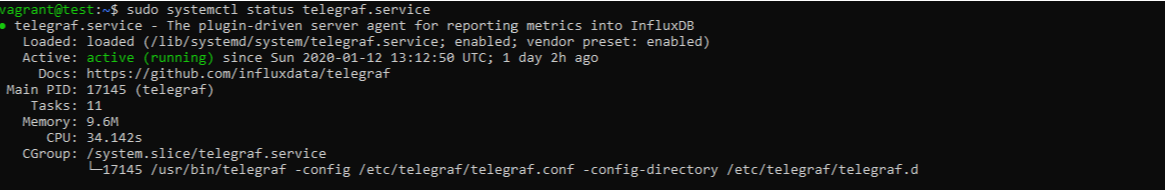
\includegraphics[width=\linewidth]{telegrafd.png}
			\caption{\texttt{Telegraf}'s Daemon Status}
			\label{f:telegrafd}
		\end{figure}
    \newpar
	With all these services running we can create awesome monitoring stations with ease. Yay \texttt{OpenSource}!

\newpage
\section{Mininet's CLI (\textbf{C}ommand \textbf{L}ine \textbf{I}nterface)}
	We've already set up our scenario and verified that it's working properly. We will now detail the most important commands we can issue from of \textbf{Mininet's CLI}.

	\subsection{Command: \texttt{EOF} + \texttt{quit} + \texttt{exit}}
		These three commands are used for the same thing, to exit the \textbf{Mininet CLI} and finish the emulation. The source code of these three commands does not differ much, \textbf{EOF} and \textbf{quit} end up using the \texttt{do\_exit} function at the end, so we could say that they are a bit repetitive. They offer several ways to kill the emulation so that people with different backgrounds feel "at \texttt{~}". The source code taking care of exiting is:

		\begin{minted}{python}
	def do_exit( self, _line ):
		"Exit"
		assert self # satisfy pylint and allow override
		return 'exited by user command'

	def do_quit( self, line ):
		"Exit"
		return self.do_exit( line )

	def do_EOF( self, line ):
		"Exit"
		output( '\n' )
		return self.do_exit( line )
		\end{minted}

	\subsection{Command: \texttt{dpctl}}
		The \textbf{dpctl} command is a management utility that allows some control over the OpenFlow switch (ovs-ofctl on the OpenvSwitch). This tool lets us add flows to the flow table, check the features and status of the switches or clean the table among many other things. For example, recall how we previously made a ping between \textbf{h1} and \textbf{h3}. If we consult the flow tables we will be able to check how the rules for handling \textbf{ICMP} flows have been instantiated as seen in figure \ref{f:dpctl}.

		\begin{figure}[!htb]
			\centering
			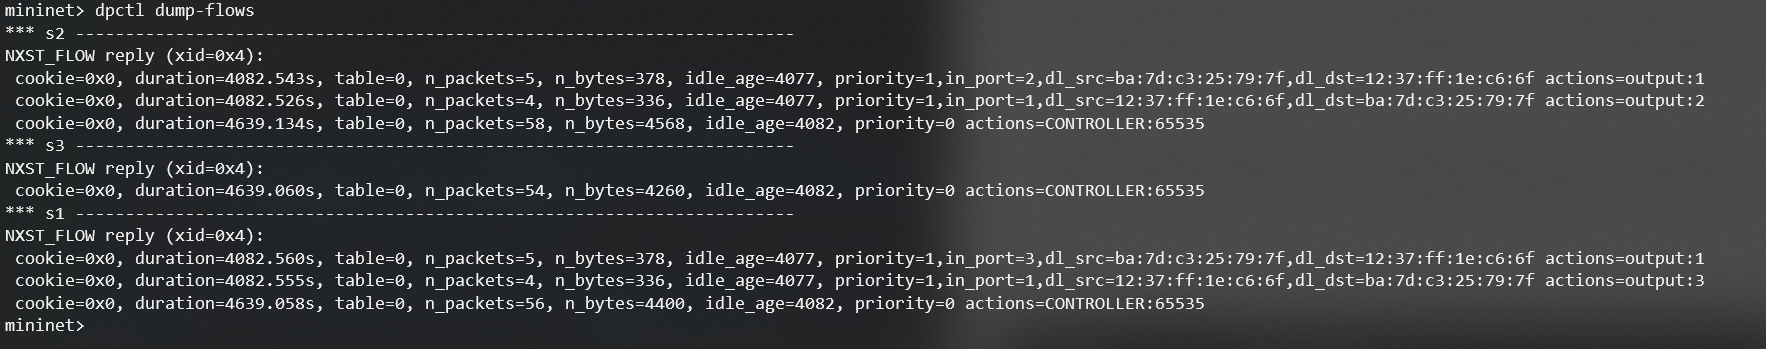
\includegraphics[width=\linewidth]{dpctl.png}
			\caption{\texttt{DumpCTL}}
			\label{f:dpctl}
		\end{figure}

		Note how in the first and third switches we have 3 flow instead of the default one that let's us communicate with the controller. On top of that, take a closer look at the third switch and notice how the input and output ports for the first flow are 3 and 1 respectively. The second rule has the exact opposite distribution: the input port is 1 and the output is port 3. This setup let's us establish a communication link through this switch between any machines hooked to port's 1 and 3. These are the rules the controller has automagically set for us!
		\newpar
		This command is quite complex and powerful, and it may not be completely necessary for what we are going to do in this practice. It is nevertheless undoubtedly one of the most important commands to understand the internal workings of \textbf{SDN} switches. For more information, we encourage you to take a look at the documentation over at \href{http://www.openvswitch.org/support/dist-docs/ovs-ofctl.8.txt}{OpenVSwitch}.

	\subsection{Command: \texttt{dump} + \texttt{net}}
		These commands will give us information about the emulated topology. The \textbf{net} command will indicate the names of the entities in the emulated topology as well as their interfaces. The \textbf{dump} command will also indicate the type of entity, its \textbf{IP} address, port when applicable, interface and the entity's process identifier (\textbf{PID}). You can find a sample output in figure \ref{f:dump}.

        \newpage
		\begin{figure}[!htb]
			\centering
			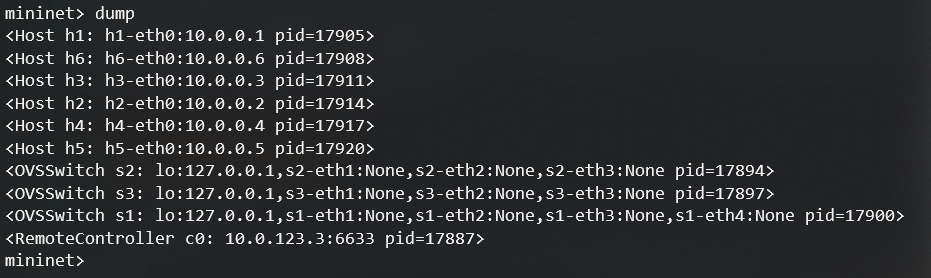
\includegraphics[width=\linewidth]{dump.png}
			\caption{\texttt{dump's} output}
			\label{f:dump}
		\end{figure}

	\subsection{Command: \texttt{xterm} + \texttt{gterm}}
		These two commands will allow us to open terminal emulators in the node identified by the accompanying argument. The command \textbf{xterm} will allow us to open a simple \textbf{XTERM} (the default terminal emulator for the \textbf{X} windows system) terminal emulator, and \textbf{gterm} launches a prettier but more resource hungry \textbf{Gnome terminal}.
		\newpar
		We can open several terminals at once by indicating all the nodes we want to open a terminal in. Later, when we discuss the inner workings of \textbf{Mininet}, we'll talk a bit more about where the \textbf{bash} process attached to the terminal emulator is running. You might think that this process is totally isolated from the machine on which you are running \textbf{Mininet}, but this is not entirely the case... You can find a \texttt{xterm} instance running in figure \ref{f:xterm}.
        \newpar
		\begin{minted}{bash}
	# xterm/gterm [node1] [node2]
	xterm h1 h6
		\end{minted}
        \newpage
		\begin{figure}[!htb]
			\centering
			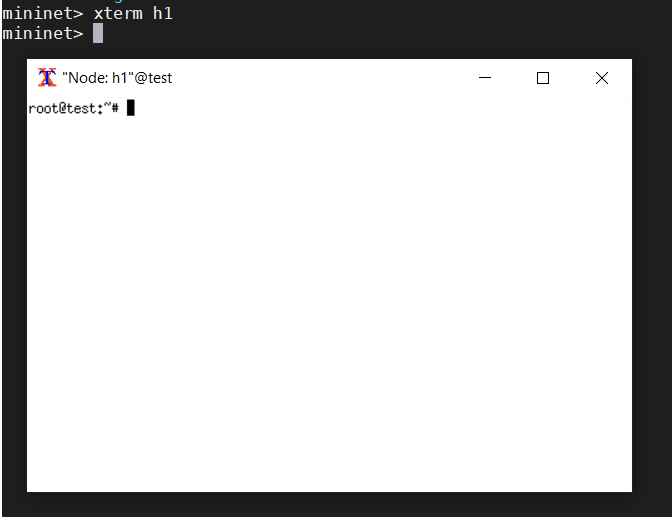
\includegraphics[width=\linewidth]{xterm.png}
			\caption{Launching \texttt{xterm} on the nodes}
			\label{f:xterm}
		\end{figure}

	\subsection{Command: \texttt{nodes} + \texttt{ports} + \texttt{initfs}}
		These commands will list information related to the nodes in the topology. The \textbf{intfs} command will list all information related to the nodes' interfaces. The  \textbf{nodes} command will show every node in the topology. Finally, the \textbf{ports} command is used to list the ports and interfaces of the switches in the topology. An example output can be found in figure \ref{f:initfs}.
        
        \newpage
		\begin{figure}[!htb]
			\centering
			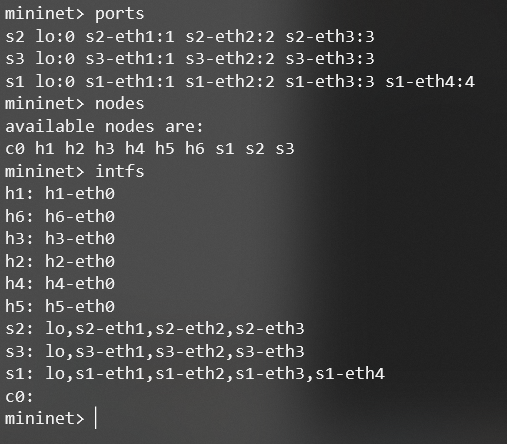
\includegraphics[width=\linewidth]{initfs_cmd.png}
			\caption{The \texttt{ports} and \texttt{initfs} commands}
			\label{f:initfs}
		\end{figure}

	\subsection{The Rest of the Commands}
		Someone once told me \textbf{manpages} were my friends. This doesn't apply here directly but you get the idea. If you don't know what a command does try running it without arguments and you will be presented with a help section hopefully. If your machine blows up... It wasn't our fault! (It really shouldn't though  ). You can also issue \texttt{help <command\_name>} from the \textbf{mininet CLI} to gather more intel. You can also contact us directly. We didn't want this section to grow too large and we believe the above commands are more than enough for our purposes.

\section{Mininet's Internals}
	We have been covering \textbf{Mininet} for a while now but... What is exactly \textbf{Mininet}? It is a tool used for emulating \textbf{SDN} (\textbf{S}oftware \textbf{D}efined \textbf{N}etworks). We can write software programs describing the network topology we want and then run them to create a virtual network just like the one we described. Cool right?
	\newpar
	Now, notice how we used the term \textbf{emulation} instead of \textbf{simulation}. Even though many people regard these terms as equivalent they are \textbf{NOT} the same. When we talk about \textbf{simulation} we are referring to software that computes the outcome of an event given an expected behaviour. On the other hand, \textbf{emulation} recreates the scenario under study in its entirety on specific hardware to then study its behaviour.
	\newpar
	An example to differentiate the two could be to think about a plane cockpit. If we were to play a video-game like \textbf{Flight Simulator} we would be simulating (no surprise) the flight but if we were to practice using a 1:1 scale with real controls we would then be talking about emulation.

	\begin{figure}[!htb]
		\centering
		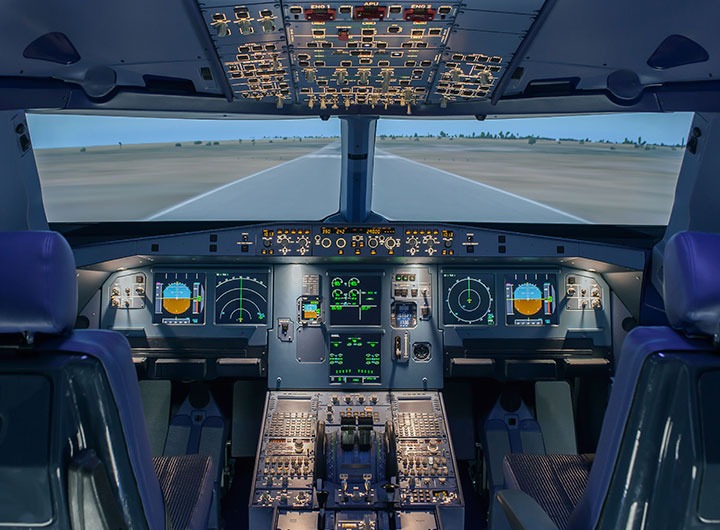
\includegraphics[width=0.7\linewidth]{emulation.png}
		\caption{A videogame portraying a flight emulator}
		\label{f:emulator}
	\end{figure}

	With this little detail out of the way we could ask ourselves. Does \textbf{mininet} emulate or simulate a network?. It is a network \textbf{emulator}, here's why. Mininet reserves system resources for each node in the \textbf{emulated} network. You might think these nodes are "just" VMs or virtualized containers but... they're not.
	
	\newpar
	That solution would have many advantages but it wouldn't scale to be able to \textbf{emulate} large networks or huge amounts of traffic as it would exhaust the host system's resources... The Mininet developers then chose to \textbf{exclusively virtualize} what was necessary to carry out the desired \textbf{network emulation}.
	\newpar
	How did they do it? By using the \textbf{Network Namespaces}.

	\subsection{Network Namespaces}
		A \textbf{network namespace} consists of a logical network stack replica that by default is composed of the \textbf{Linux kernel}, paths, \textbf{ARP} tables, \textbf{Iptables} and network interfaces.
		\newpar
		Linux starts with a default \textbf{Network namespace} which is the one everyday users need for example. This namespace includes a routing table, an ARP table, the iptables and any network interfaces it might need. The key here is that it is also possible to create more non-default network namespaces. We can then create new devices in those namespaces, or move an existing devices from one namespace to another. This is a rather complex virtualization concept provided by the Linux kernel and we will not delve any further. It is quite interesting if you ask us though...
		\newpar
		In this way, each network element has its own network namespace, i.e. each element has its own network stack and interfaces. So at the networking level, one could say, they are independent elements. The key is that every node shares the same process namespace, IPCs namespace, filesystem... We are virtualizing up to the network layer only. This is the true power of the network stack approach to things. As Vegeta would put it: "The network namespace's power is over 9000!" just like we see him say in figure \ref{f:ns_power}.

		\begin{figure}[!htb]
			\centering
			
\includegraphics[width=0.6\linewidth]{vegeta.png}
			\caption{The namespaces' power is...}
			\label{f:ns_power}
		\end{figure}
        
        \newpar
		In figure \ref{f:x_htop} we can see how we created a process in the host machine with the \texttt{sleep} command whose \textbf{PID} is \texttt{20483}. If the network elements were really isolated we wouldn't be able to see this process from other machines but the reality is different with mininet as we discussed.
		\newpar
		This is something to assume when working with Mininet's low-cost emulation. This approach would be lacking in other scenarios but it is more than enough to emulate a network. This fact casts some doubts on how to integrate our data collection system with \textbf{telegraf} in the different network elements without any incompatibilities...
		\newpar
		That's why we decided to take the controller "out of" the machine where Mininet was going to run so as to avoid problems with by-passes by IPCs from telegraf to the InfluxDB database. The only thing left for us to do is to figure out how to correctly install and configure telegraf so that everything works as intended.
		\newpage

		\begin{figure}[!htb]
			\centering
			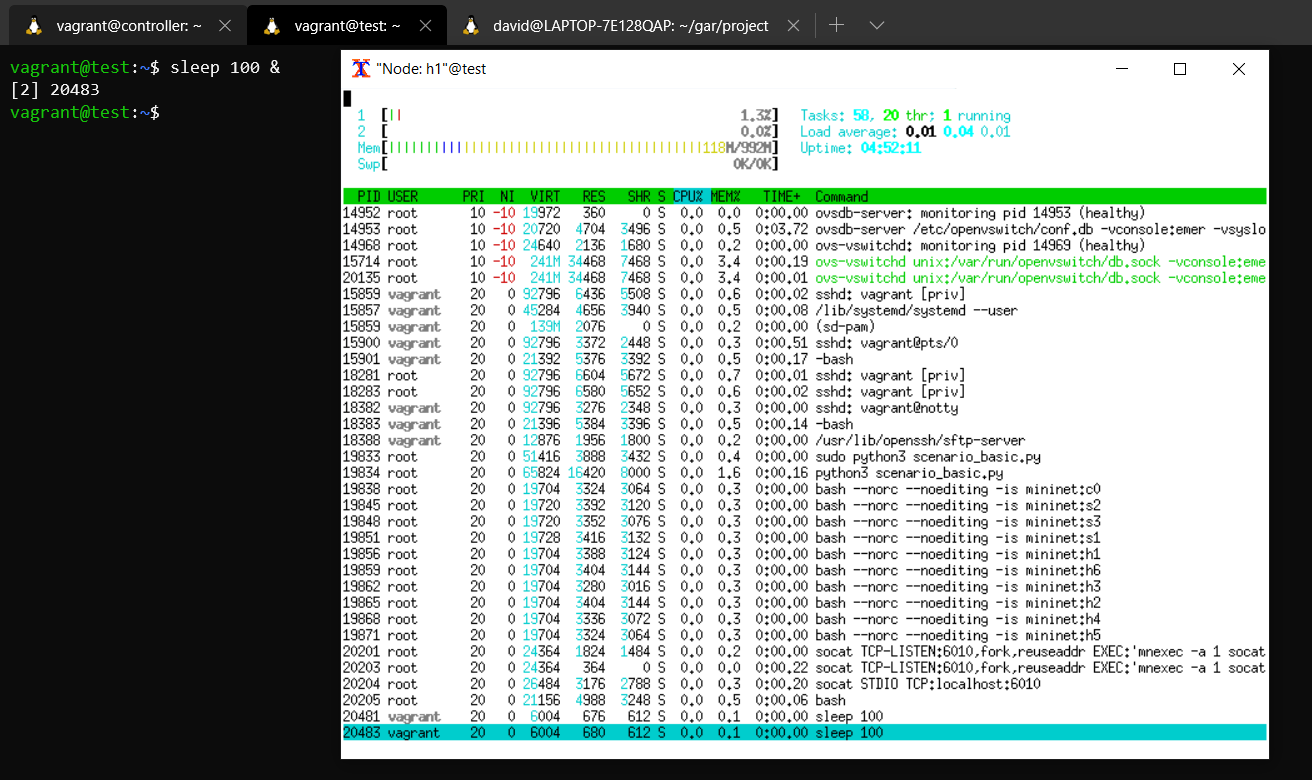
\includegraphics[width=\linewidth]{x_htop.png}
			\caption{A lazy process...}
			\label{f:x_htop}
		\end{figure}

\newpage

\section{Mininet's Internals (II)}
	In this second part on the internal operation of Mininet, we will investigate the Kernel-level topology recreated by Mininet to set up our scenario. Finally, we will explain the different ways to raise services in the different Network namespaces, necessary to collect information with \texttt{telegraf}. 

	\subsection{Is Mininet Actually Using Namespaces?}
		We have previously introduced that Mininet makes use of Network namespaces as a method to virtualize network stacks independent of each other, so that we can emulate networks at a minimum cost, but how can we be so sure that it really makes use of them? Here are the steps to verify whether or not Mininet is using Network namespaces.
		\newpar
		The first thing we have to do is run the scenario so that mininet can create the network namespaces that it needs to create. In addition, we can also run the controller in the controller machine to check at the last moment that none of the checks made have affected the operation of our scenario.

		\begin{minted}{bash}
	# On the test machine, to set up the topology.
	sudo python3 scenario_basic.py

	# On the controller machine, to run the controller
	ryu-manager ryu.app.simple_switch_13
		\end{minted}

		Now that we've set the scenario up we should be able to see if there are any Network namespaces on our machine, to do this we'll use the \textbf{iproute2} toolkit. Within this pack we will keep the most famous tool, \texttt{ip}. The \texttt{ip} tool is becoming established in the new Linux distributions as the de facto tool to work on everything related to Networking in a Linux environment. In the latest versions of Ubuntu for example, the \texttt{ifconfig} command is starting to be replaced by the iproute2 toolkit (a.k.a \texttt{ip}). This tool has many modules, for more information see its manual:

		\begin{itemize}
			\item Tool's manual: \href{https://linux.die.net/man/8/ip}{\texttt{ip}}
		\end{itemize}

		The module that we will need to work with Network namespaces is \textbf{netns}, we can see all that it can offer us by doing \texttt{ip netns help}. The main command to list the Network namespaces using the netns module is the following:

		\begin{minted}{bash}
	sudo ip netns list
		\end{minted}

		Knowing the command to list Network Namespaces, and having previously set up the scenario, we'll check if there really are any Network Namespaces created on our machine in figure \ref{f:netns_list}.

		\begin{figure}[!htb]
			\centering
			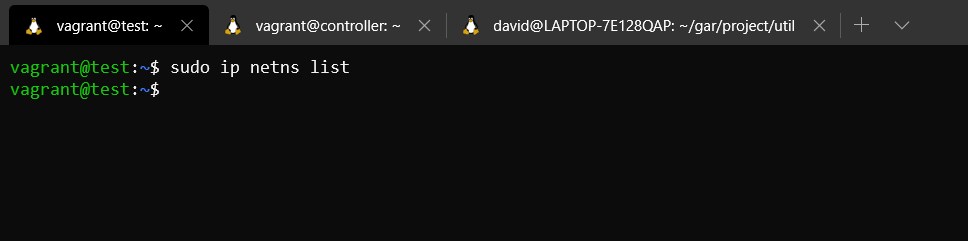
\includegraphics[width=\linewidth]{netns_list.png}
			\label{f:netns_list}
			\caption{Listing the network namespaces}
		\end{figure}

		After checking figure \ref{f:netns_list} it seems that there is no Network namespace created, maybe, \textbf{Mininet doesn't work as we said before?} First of all, let's calm down just like \textbf{Tux} in figure \ref{f:tux}, we don't have to rewrite all the documentation.

		\begin{figure}[!htb]
			\centering
			
\includegraphics[width=0.6\linewidth]{calm_tux.jpg}
			\label{f:tux}
			\caption{Just chilling}
		\end{figure}

		\subsubsection{Not Today!}
			The problem that the command \texttt{ip netns list} \textbf{doesn't} give us information, is that mininet is not creating the required softlink for the tool to be able to list the network namespaces, if we read the \href{http://man7.org/linux/man-pages/man8/ip-netns.8.html}{documentation} we can find out that \texttt{ip netns list} reads from the path \texttt{/var/run/netns/} where all the named network namespaces are placed. 
			\newpar
			If you've gotten to this point you probably want to check that iproute2 really does read from where it says it reads. We can get a trace of the system, i.e. collect all the syscalls made by a program and debug them ourselves. To do this we will use the \texttt{strace} command. For more information see their \href{https://linux.die.net/man/1/strace}{manual}. The command we will use to get the syscalls trace is the following:

			\begin{minted}{bash}
	sudo starce ip netns list
			\end{minted}

			Then the output obtained will be like the one in figure \ref{f:sys_trace} (try to zoom in on the image).

			\begin{figure}[!htb]
				\centering
				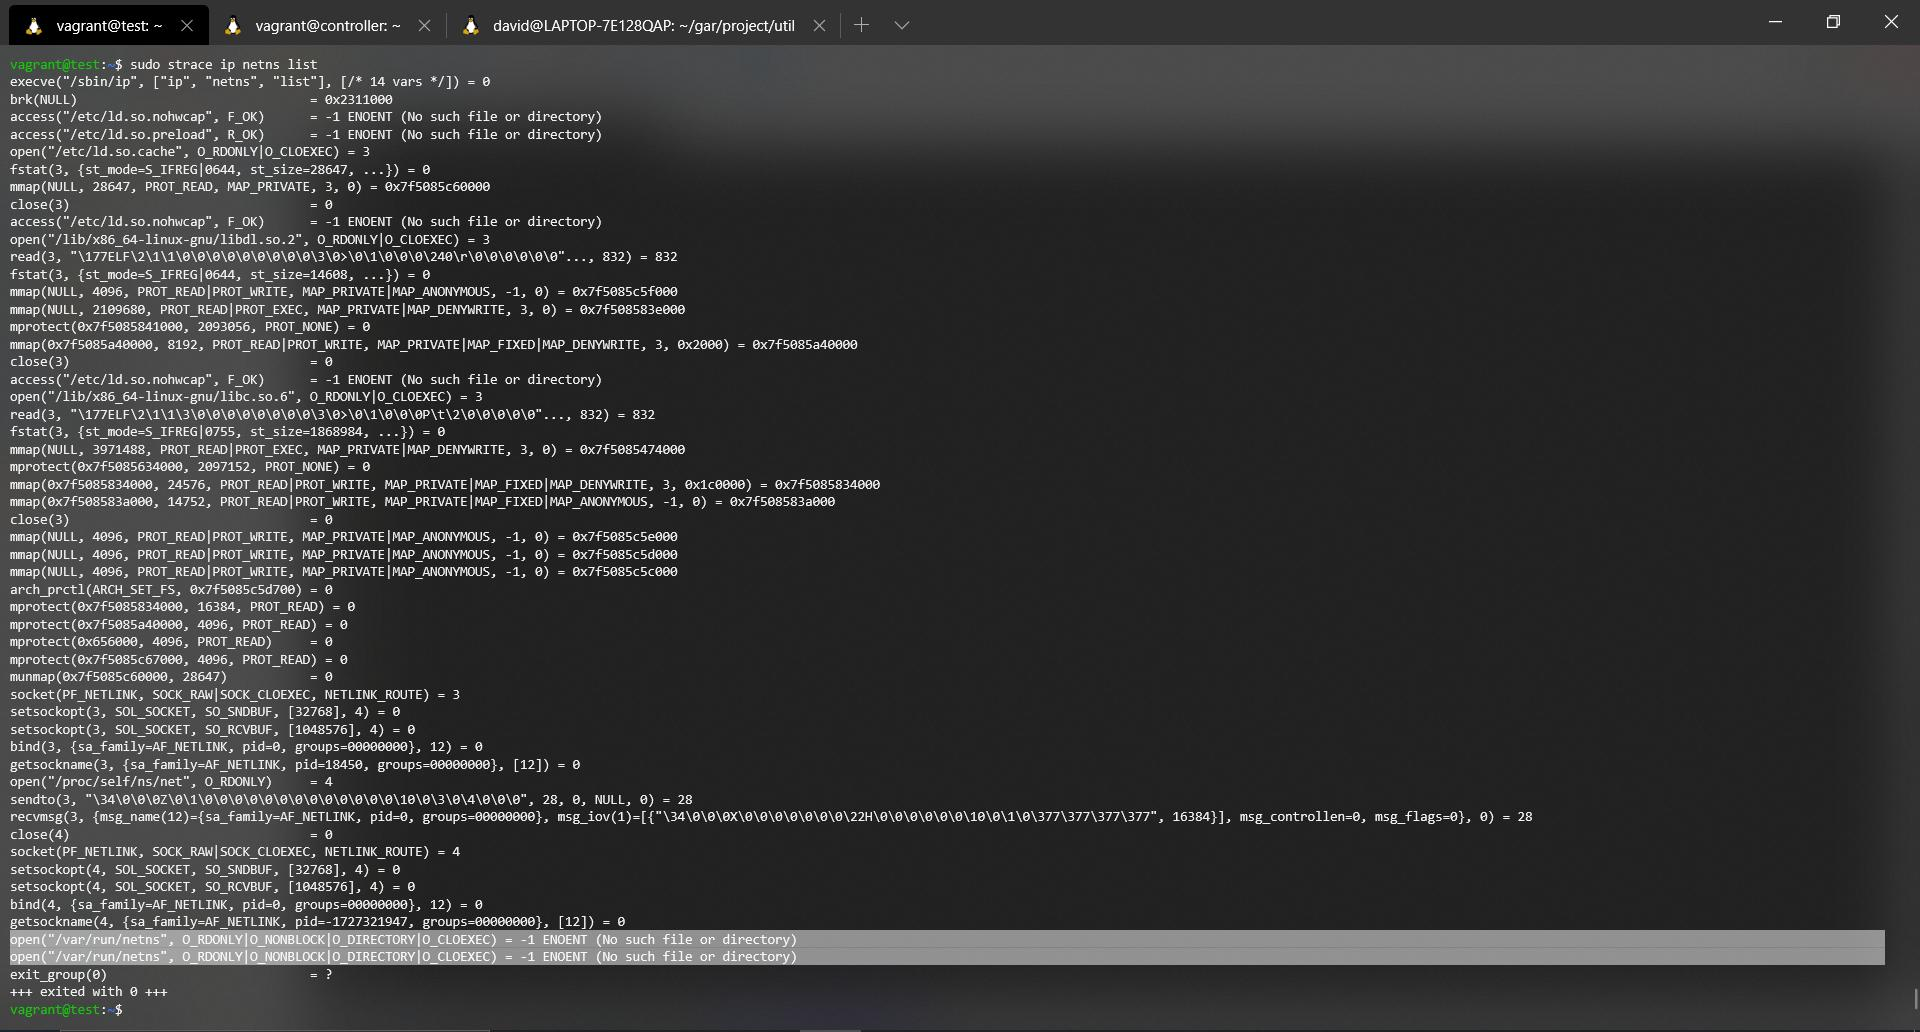
\includegraphics[width=\linewidth]{sys_trace.jpg}
				\label{f:sys_trace}
				\caption{Systrace's output}
			\end{figure}

			Let's take a good look at the last four lines from figure \ref{f:sys_trace}. If it doesn't look right in the picture, it's these lines:

			\begin{minted}{c}
	open("/var/run/netns", O_RDONLY|O_NONBLOCK|O_DIRECTORY|
	O_CLOEXEC) = -1 ENOENT (No such file or directory)
	exit_group(0) = ?
	+++ exited with 0 +++
			\end{minted}

			The first part of the trace is going to be omitted since the only thing it does is, parse the parameters introduced, load very basic dynamic library functions in Linux (\texttt{*.so} files, shared objects, for example, cache, libc among others). We will keep the last lines of the trace where you can see perfectly how it tries to make an \texttt{open}, in read mode of the directory, but this \textbf{does not exist}.
			\newpar
			So we can say that the \texttt{ip netns list} command does work correctly. But then, where are the network namespaces used by Mininet?

		\subsubsection{So where are Mininet's Network Namespaces located?}
			Well, to answer this question, we must first understand one thing. The \texttt{ip} tool with its \textbf{netns} module acts as a wrapper when we work with Network namespaces. Namespaces (there are several \href{http://man7.org/linux/man-pages/man7/network_namespaces.7.html}{types}) have a finite life, that is, they live as long as they are \textbf{referenced}. A namespace can be referenced in \textbf{three} ways:

			\begin{itemize}
				\item As long as there's \textbf{a process running} inside this namespace.
				\item As long as you have opened a file descriptor to the namespace file. (\texttt{/proc/{pid}/ns/{type\_namespace}})
				\item As long as there is a bind mount of the file (\texttt{/proc/{pid}/ns/{namespace type}}) of the namespace in question.
			\end{itemize}

			If none of these conditions are met, the namespace in question is \textbf{deleted}. If it is a \texttt{net} type namespace (a.k.a Network Namespace) those interfaces that are in the disappearing namespace will return to the default namespace. Once we understand this concept, we must think about the nature of the Network namespaces that Mininet creates.
			\newpar
			Mininet, when is launched it creates an emulated network, when is closed it should disappear, this process should be as light and fast as possible to provide a better user experience. The nature of Mininet's needs leads us to believe that the creation and destruction of network namespaces is associated with the first condition of referencing a namespace. 
			\newpar
			
			That is, there would be no point in making mounts or softlinks that will have to be removed later, as this would mean a significant workload for large network emulations and an increase in the time spent cleaning up the system once the emulation is complete. In addition, we must take into account that there is a third condition that is quite suitable with Mininet's needs, since only one process is needed running per Network namespace, and when cleaning we must only finish with the processes that \textit{support} the Network namespaces.
            \newpar
            
		\subsubsection{Just a hypothesis?}
			Well, according to the above reasoning, we should see several processes that are created at the time of the build-up of our scenario in Mininet. These processes should each have a Network Namespace file, \texttt{/proc/{pid}/ns/net}, with a different \textbf{inode} for those processes running in different Network namespaces. Where do we start looking?
            \newpar
			Let's set the scenario up if we haven't set it up before, list all processes, and filter by the name of \textit{mininet}. Let's see what we find.
			\newpar

			\begin{minted}{bash}
	sudo ps aux | grep mininet
			\end{minted}

			The output of the avobe command can be seen in figure \ref{f:netns_procs}.
            \newpage
			\begin{figure}[!htb]
				\centering
				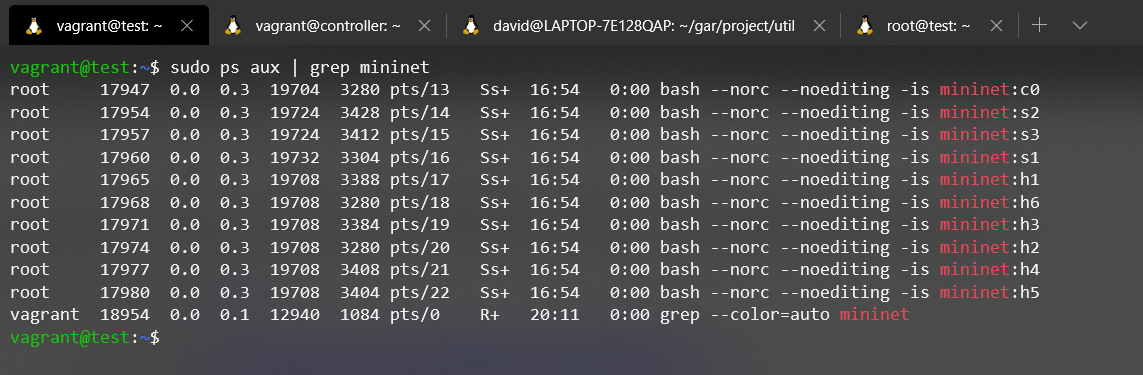
\includegraphics[width=\linewidth]{netns_procs.png}
				\label{f:netns_procs}
				\caption{Mininet's processes}
			\end{figure}

			Wow! Without having created any process associated with each node in our scenario, there is already a process running a bash associated with each element in the scenario at the start of the emulation. That's funny... Isn't it? Let's dig a little deeper.
			\newpar
			If we inspect the \texttt{/proc/{pid}/ns/net} file for each process we can see which ones are in a different network namespace depending on the value of the inode. For example, let's check the processes associated to hosts 1 and 2 can be seen in figures \ref{f:host1_procs} and \ref{f:host2_procs} respectively.
            \newpar
            
			\begin{figure}[!htb]
				\centering
				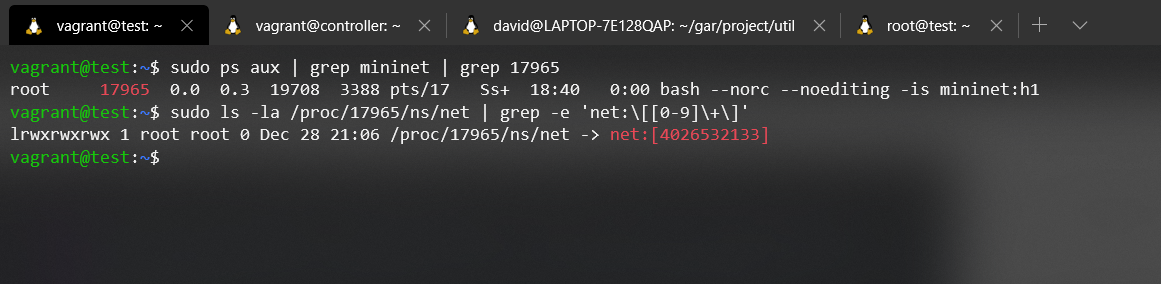
\includegraphics[width=\linewidth]{host1_procs.png}
				\label{f:host1_procs}
				\caption{Host1's processes}
			\end{figure}
            \newpage
			\begin{figure}[!htb]
				\centering
				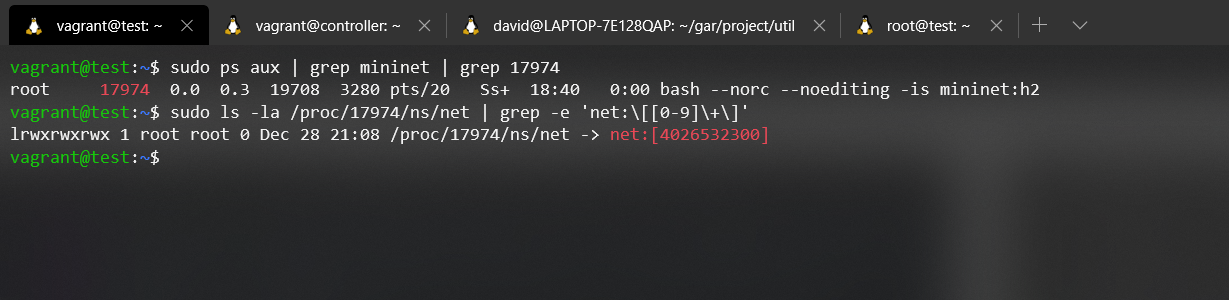
\includegraphics[width=\linewidth]{host2_procs.png}
				\label{f:host2_procs}
				\caption{Hosts2's processes}
			\end{figure}

			As you can see, different inodes, different files, \textbf{different network namespaces}. In order to make it more evident, we are going to execute a command to show which interfaces are associated to each Network namespace. In order to inject processes into a namespace we will use the \texttt{nsenter} tool. For more information about this tool, please refer to its \href{http://man7.org/linux/man-pages/man1/nsenter.1.html}{manual}.
            	\newpar
			\begin{minted}{bash}
	nsenter --target <pid> --net {Command}
			\end{minted}
            \newpar
			The output of the above command for hosts 1 and 2 can be seen in figures \ref{f:host1_intf} and \ref{f:host2_intf} respectively.
		

			\begin{figure}[!htb]
				\centering
				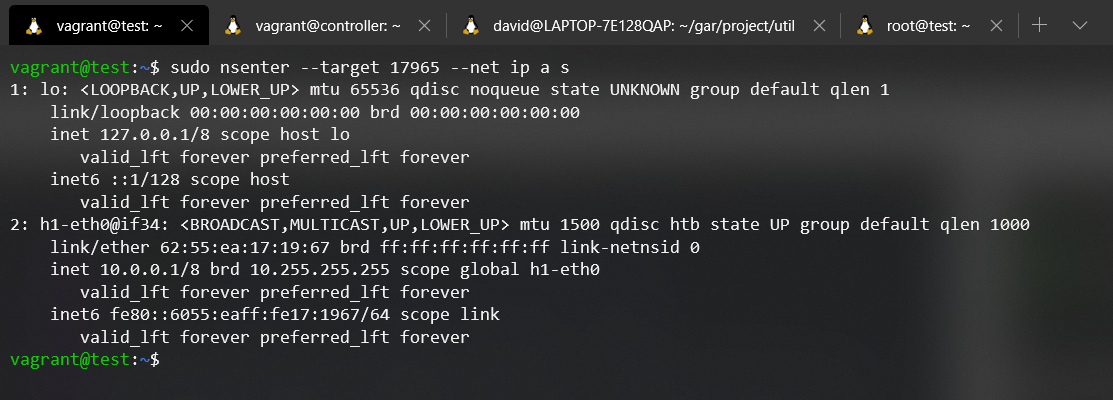
\includegraphics[width=\linewidth]{host1_intf.png}
				\label{f:host1_intf}
				\caption{Running \texttt{ip} on another Host1's namespace}
			\end{figure}

			\begin{figure}[!htb]
				\centering
				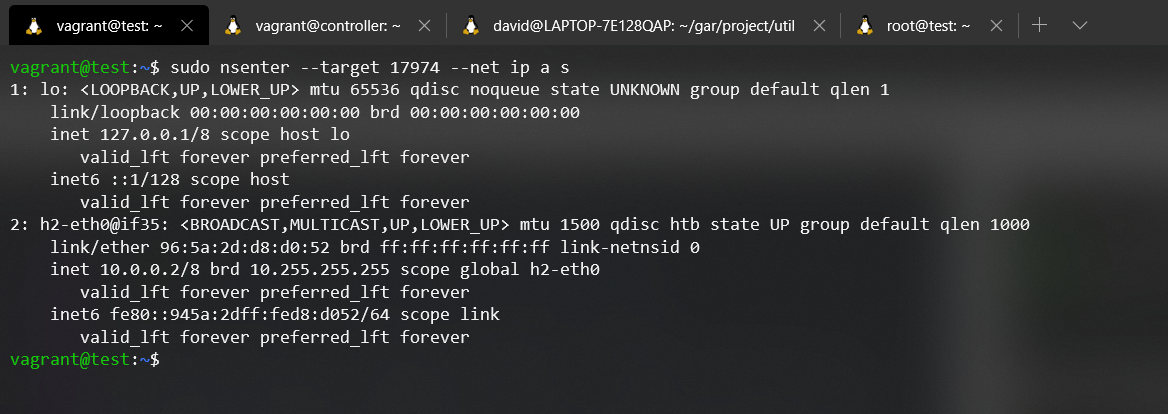
\includegraphics[width=\linewidth]{host2_intf.png}
				\label{f:host2_intf}
				\caption{Running \texttt{ip} on another Host2's namespace}
			\end{figure}

			If we look at the command entered in each network namespace it is the same, \texttt{ip addr show} (a.k.a \texttt{ip a s}). With this command we can list all the addresses assigned to each interface of the Network namespace. The result obtained from the execution of each command is the expected one, in the Network namespace of the \textbf{Host1} we can see that the interface \texttt{h1-eth0} exists, and in the Network namespace of the \textbf{Host2} the interface \texttt{h2-eth0}. With this test we conclude with the existence of the Network namespace that Mininet uses.
			\newpar
			Additionally we can corroborate our hypothesis by changing the "\textit{verbosity}" of our script,  where we build the whole scenario topology, \newline \href{https://github.com/GAR-Project/project/blob/master/src/scenario_basic.py}{\texttt{src/scenario\_basic.py}}, we can change the level of \texttt{info} to \texttt{debug}, and launch the script again.

			\begin{minted}{python}
	if __name__ == '__main__':
		#setLogLevel('info')
		setLogLevel('debug')
		scenario_basic()
			\end{minted}

			\begin{figure}
				\centering
				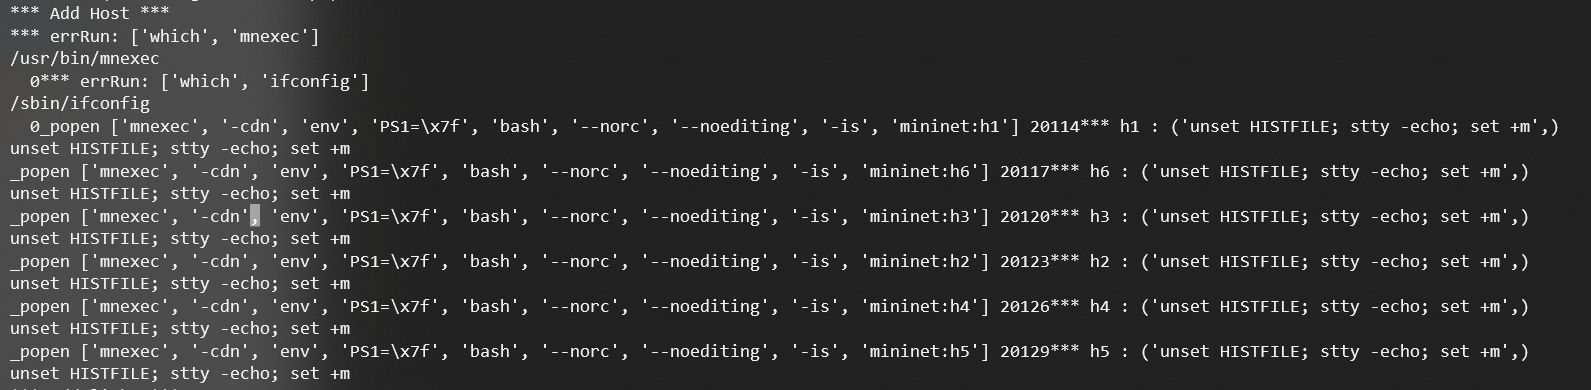
\includegraphics[width=\linewidth]{debug.png}
				\label{f:debug}
				\caption{Mininet's debugging information}
			\end{figure}

			As you can see in the execution output from figure \ref{f:debug}, \texttt{veth} is created (\textbf{V}virtual \textbf{Eth}ernet devices), and the different processes that \textit{will} support the different Network Namespaces. Furthermore, it has been possible to check how the \texttt{tc} (\textbf{T}raffic \textbf{C}controller) is used to establish the bandwidth and maximum queue limits to the links in the scenario.

		\subsubsection{So, is it possible to use \texttt{iproute2} with Mininet?}
			The quick and easy answer in the current state would be that \textbf{no}. We can always make use of the Python API to run things inside a network element or if not, we can ultimately open the Mininet CLI, open an xterm and throw things by hand, or as we have done before make use of the \texttt{nsenter} tool. 
			\newpar
			So, there is no solution ? Well, almost everything has a solution, it depends on us to how far we want to go to fix things. Let's see how we can enable the Network namespace of \textbf{Host1} to be visible for \texttt{ip netns}. First we must locate the PID of the bash that holds the Host1 Network Namespace. In our case it is the following:

			\begin{minted}{bash}
	sudo ps aux | grep mininet | grep h1
			\end{minted}

			The output of the avobe command can be seen in figure \ref{f:h1_pid}.

			\begin{figure}[!htb]
				\centering
				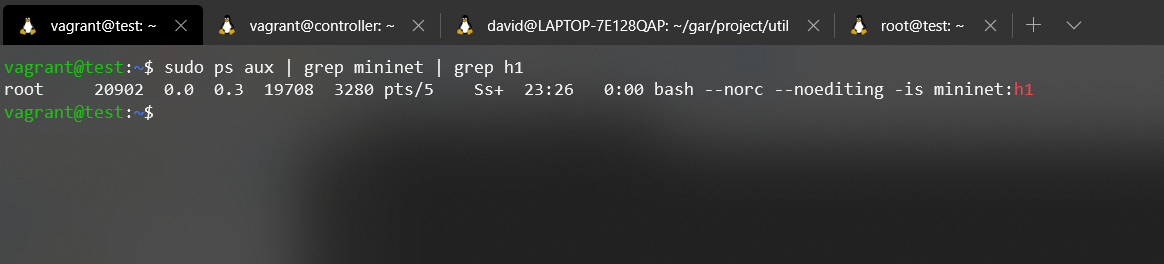
\includegraphics[width=\linewidth]{h1_pid.png}
				\label{f:h1_pid}
				\caption{Getting Host1's processes again}
			\end{figure}

			Once we know the PID of the process that \textit{holds} the Host1 Network Namespace, we will create the \texttt{/var/run/netns} directory in case it is not created:

			\begin{minted}{bash}
	# We use the -p parameter so that in case it exists
	# it does not give us errors.
	mkdir -p /var/run/netns/
			\end{minted}

			We must make a softlink from the original Network Namespace file in the created directory (Let's remember that this is the path where the \texttt{ip netns list} command reads from).

			\begin{minted}{bash}
	sudo ln -sfT /proc/<PID>/ns/net /var/run/netns/h1
			\end{minted}

			The output of the above command can be seen in figure \ref{f:lnk}.

			\begin{figure}[!htb]
				\centering
				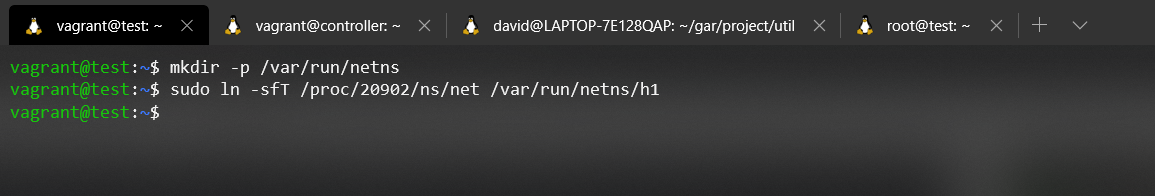
\includegraphics[width=\linewidth]{lnk.png}
				\label{f:lnk}
				\caption{Making a symbolic link}
			\end{figure}

			Finally, we would only have to try again the command 'ip netns list' to see if it is able to list the Network namespace. The output can be seen in figure \ref{f:it_works}.

			\begin{figure}[!htb]
				\centering
				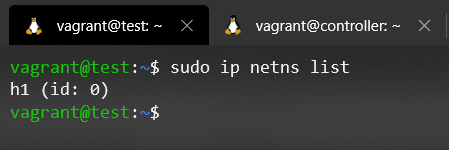
\includegraphics[width=0.7\linewidth]{it_works.png}
				\label{f:it_works}
				\caption{Listing the network namespaces once more}
			\end{figure}
                
    
			Some will say it's dark magic.. But, it's just that, creating a softlink and knowing how each element works.

			\begin{figure}[!htb]
				\centering
				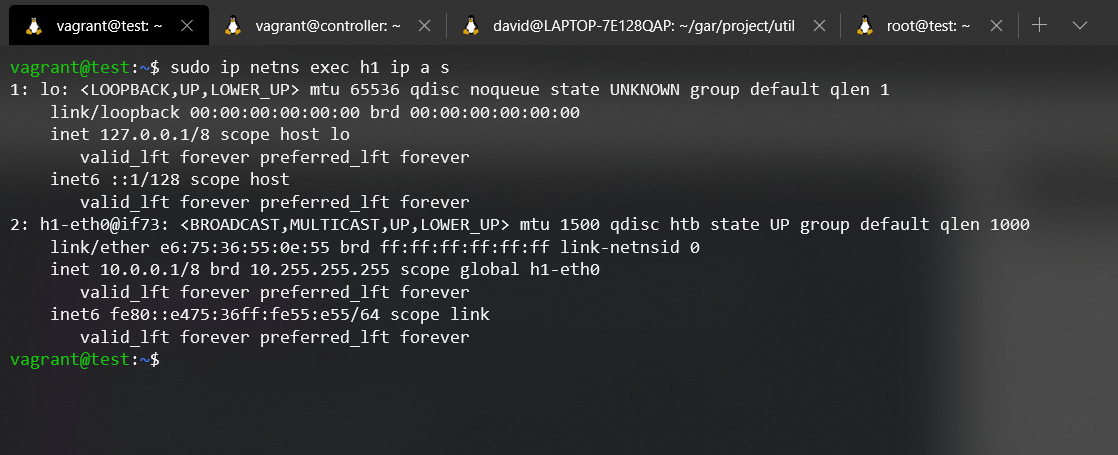
\includegraphics[width=\linewidth]{iproute2_fixed.png}
				\label{f:iproute2_fixed}
				\caption{It works!}
			\end{figure}

			As you can see in figure \ref{f:iproute2_fixed}, the command is fully functional. You can see how we are able to list all the interfaces of Host1's Network namespace. But as everything, it always has pros and cons, when we make the arrangement of creating a softlink and turning off the emulation with its corresponding system cleaning (we are mainly concerned with the elimination of the processes that supported the Network namespace), we are left with a broken softlink pointing to a site that no longer exists, or is no longer useful.
            \newpar
			\begin{figure}[!htb]
				\centering
				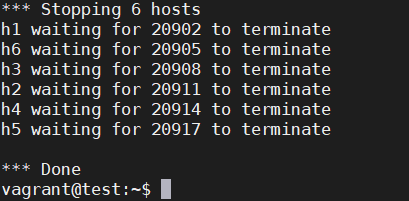
\includegraphics[width=0.8\linewidth]{shutting_down.png}
				\label{f:shutting_down}
				\caption{Shutting Mininet down}
			\end{figure}
            \newpage
			\begin{figure}[!htb]
				\centering
				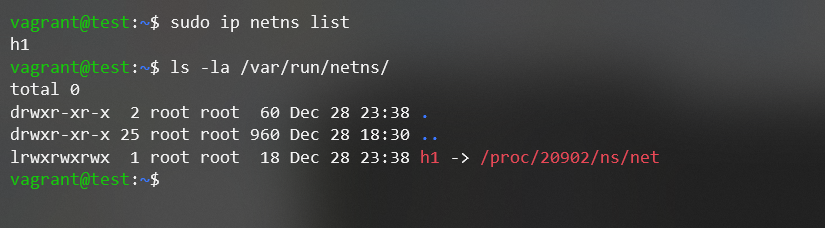
\includegraphics[width=0.9\linewidth]{broken_softlink.png}
				\label{f:broken_softlink}
				\caption{Broken Softlink}
			\end{figure}

			With the outputs shown in figures \ref{f:shutting_down} and \ref{f:broken_softlink}, it is left up to the user to decide whether or not to use the iproute2 tool. If this is the case, it is recommended that an auxiliary cleaning script be developed to clean up those softlinks that are broken in the \texttt{/var/run/netns} directory when the emulation is finished.
            
	\subsection{The Big Picture}
		Once we have concluded that Mininet makes use of Network namespaces and we know how to demonstrate it, we will inspect each of the Network namespaces to draw a scheme of how our Kernel-level scenario is implemented. Let's take another look at our scenario in figure \ref{f:scenario_prime}.

		\begin{figure}[!htb]
			\centering
			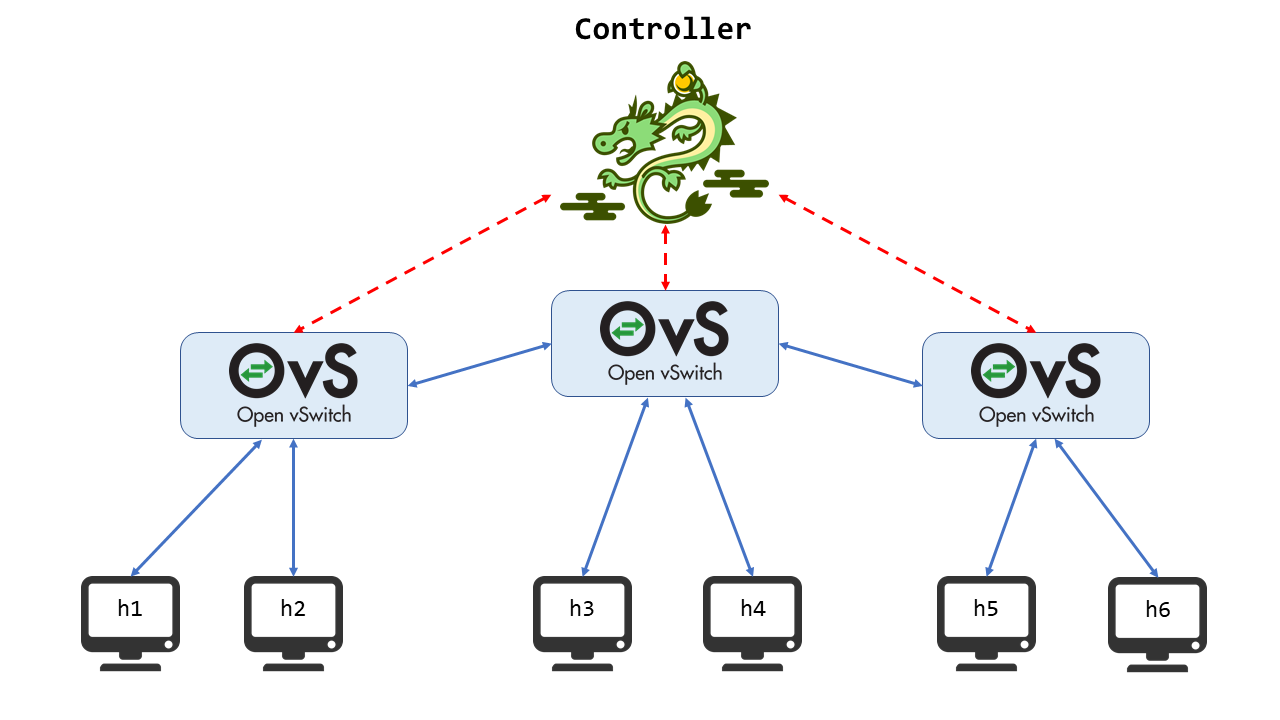
\includegraphics[width=0.8\linewidth]{scenario.png}
			\label{f:scenario_prime}
			\caption{Let's go back to the basic scenario}
		\end{figure}
        \newpage
		As you can observe in figure \ref{f:switches}, the switches are network elements that are supposed to be isolated in a network namespace, but for our surprise they are not in the default network namespace. Why does it work then, because there is no by-pass to the default network stack? This is because of the nature of veth, which goes straight to the OVS process itself. (A future guide will attempt to address this issue more fully).

		\begin{figure}[!htb]
			\centering
			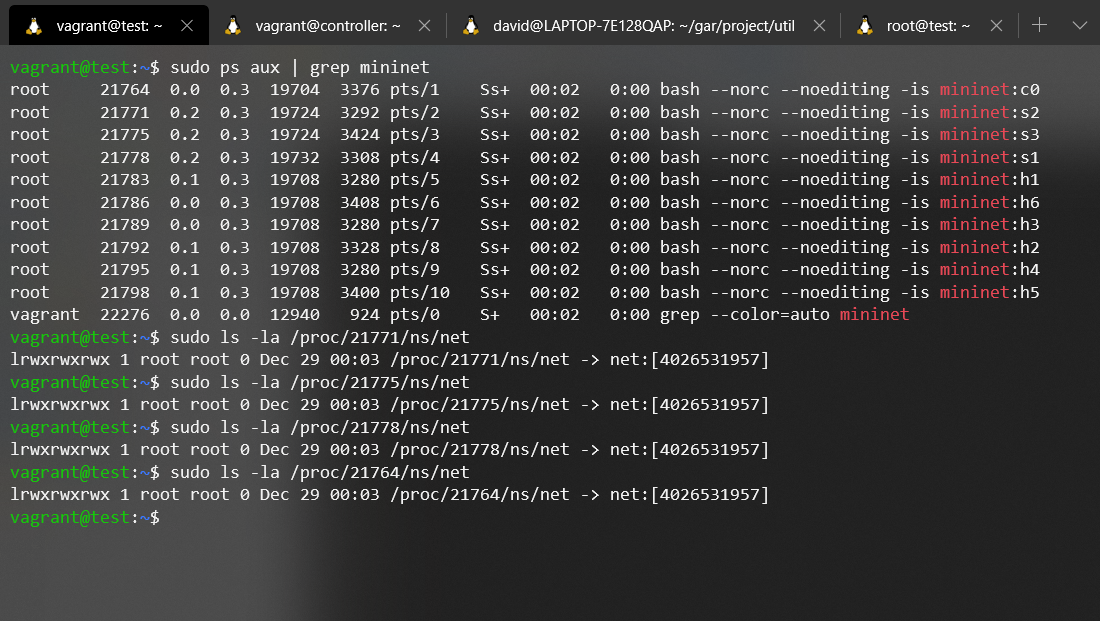
\includegraphics[width=\linewidth]{switches_ln.png}
			\label{f:switches}
			\caption{Checking the switche's processes}
		\end{figure}

		\subsubsection{How Would Our Kernel-level Scenario Look Then?}
        \newpar
		The final "scenario" can be seen in figure \ref{f:scenario_kernel}.
        \newpage
		\begin{figure}[!htb]
			\centering
			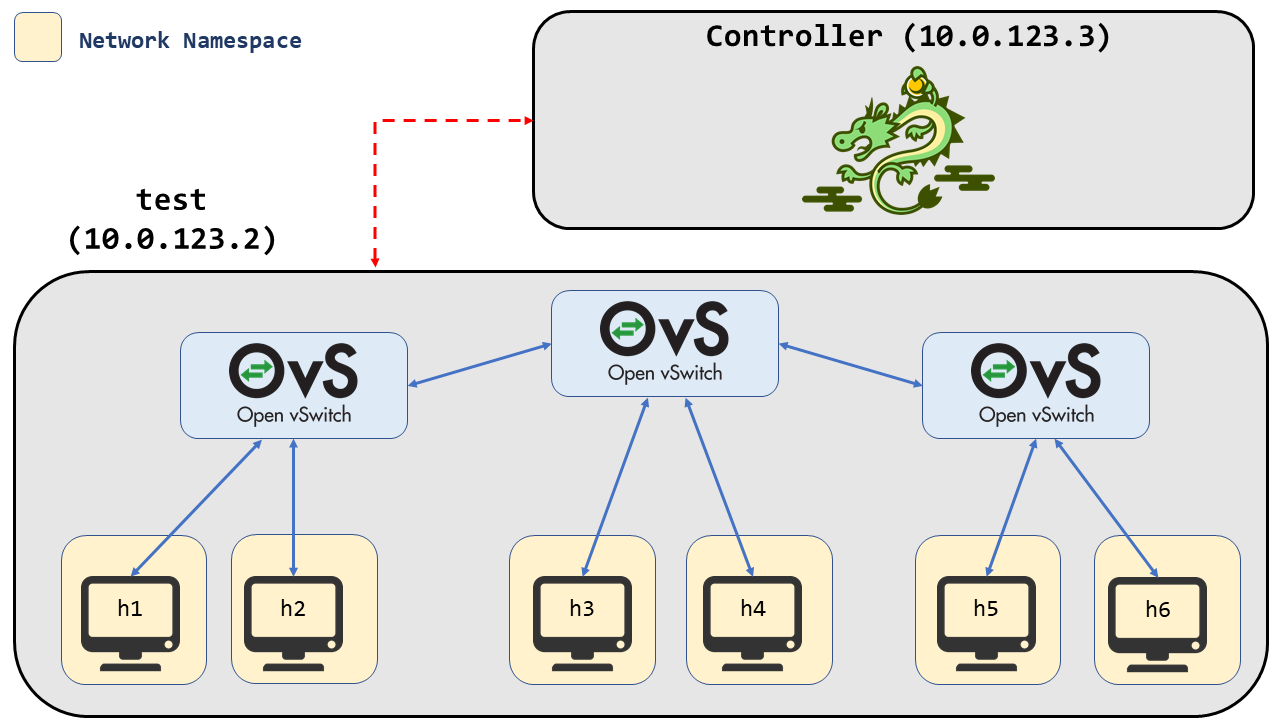
\includegraphics[width=\linewidth]{scenario_kernel.png}
			\label{f:scenario_kernel}
			\caption{Scenario taking namesapces into account}
		\end{figure}

		So, to run \texttt{telegraf} only on the switches we would just launch it on the default network namespace! This can be done with a single \texttt{telegraf} process since the useful interfaces are all in the same Network namespace.

        \newpage

\section{Troubleshooting}
	\begin{itemize}
		\item If we are to use a terminal emulator without an \textbf{X server} installed or properly configured the \textbf{miniedit} tool will not run. This tool presents us with a GUI we can use to define our network and then it'll generate a script that brings it up for us. If we are to reroute the \textbf{stdout} of a VM we will need to set the \texttt{\$DISPLAY} variable accordingly as \textbf{miniedit} used \textbf{tkinter} and it needs it to run correctly.
		\item If there are problems when launching the scenario try to clean up the previous environment. If we exit the mininet CLI by issuing the \texttt{quit} everything should be deleted correctly, otherwise we can always clean it up ourselves by running: \mint{bash}|sudo nm -c|. You can take a look at the output in figure \ref{f:mn_clean}.
	\end{itemize}

	\begin{figure}[!htb]
		\centering
		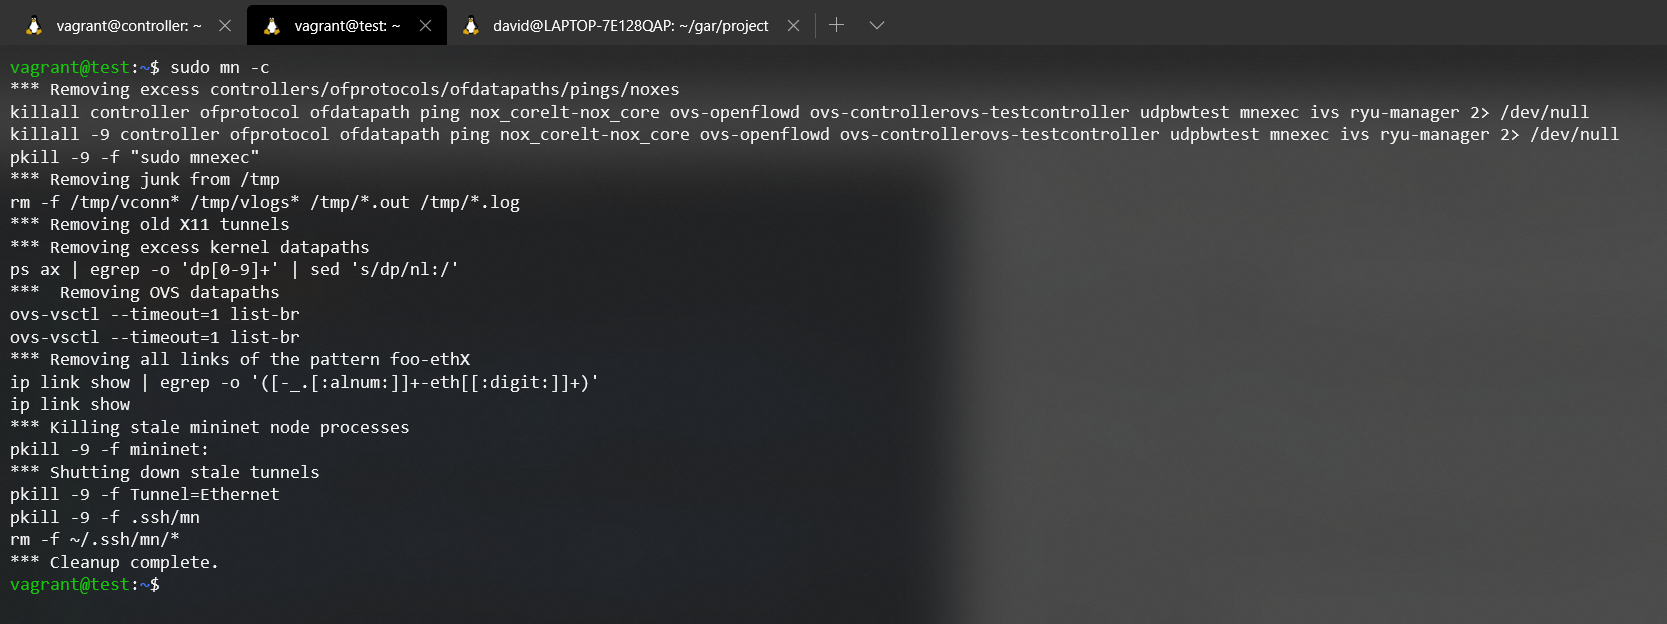
\includegraphics[width=\linewidth]{mn_clean.png}
		\label{f:mn_clean}
		\caption{"Cleaning" Mininet}
	\end{figure}

\newpage

\section{Appendix}
	We have decided to prepare an appendix so that we can shed some light on obscure topics not directly related to the project itself. We'll talk about tangential components of the project so that we can have a clearer idea of what's going on in the background and you can get a better grasp of the tools we have employed. It's a win win!

	\subsection{The Vagrantfile}
		I bet you have heard about \texttt{Virtualbox} this wonderful program lets us virtualize an entire computer inside our own so that we can try new Linux-based distros, use a Windows OS from Linux or just "create" a server farm for our own personal needs amongst many other use cases. These "virtual computers" are called \textbf{Virtual Machines} or \textbf{VM}s in \texttt{Virtualbox} lingo. The "bad" thing is that \texttt{Virtualbox} only offers a \textbf{GUI} (\textbf{G}raphical \textbf{U}ser \textbf{I}nterface) to manage new and existing VMs which makes the process extremely slow and changes it with each new update (the window titles vary, the menus are in different places...). This poses no problem at all to the average user but it becomes a nuisance in scenarios like ours.
		\newpar
		Another point of concern is the VM's provisioning: How can we get files from the host machine into the VM? We commonly used shared folders between the host machine and the VM but the set-up process can be a real pain. Is there any hope left in the galaxy? Yes: Help me \texttt{Vagrant}, you are my only hope!
		\newpar
		We can think of \texttt{Vagrant} as a wrapper for \texttt{Virtualbox} that let's us describe the VM's we want in a file called the \texttt{Vagrantfile}. We then run \texttt{Vagrant} with this file as an input and everything will be set up for us! By changing the \texttt{Vagrantfile} we can modify every VM in our topology. This includes provisioning new files, changing their memory, hostname, OS... This allows for a much more reproducible environment and hence a great portability.
		\newpar
		The \texttt{Vagrantfile} itself is written in \texttt{ruby}. It's contents are mostly in plain English and we have included comments for the tricky parts so as to make everything as clear as possible. You can even use this \texttt{Vagrantfile} as a template for your own projects!

	\subsection{File Struct: \texttt{stdout} and friends}
		What's a file struct? We can think of it as an information bundle describing a place we can write data to and read data from. We can employ these file descriptors to communicate our programs with the exterior world by means of a file. In \texttt{C} we can open files through their file descriptors which we create thanks to the \texttt{fopen()} function. If you take a closer look at the documentation you will see the type returned by \texttt{fopen()} is in fact a pointer to a \texttt{FILE struct} (i.e a \texttt{FILE*}). This \texttt{FILE struct} contains info about the file itself: Have we reached the \texttt{End Of File} mark?, where are we going to read/write with our next instruction?, has there been any error when reading/writing data? This will let us handle our file in any way we want!
		\newpar
		If you think about it we are constantly writing to the terminal from our programs using functions like \texttt{printf()} in \texttt{C} and \texttt{print()} in \texttt{python3}. Do you remember opening a file descriptor to be able to write to the terminal? I bet not! This is because our running programs are given 3 default file descriptors: \texttt{stdout}, \texttt{stdin} and \texttt{stderr}. These are connected to the terminal running the program (usually), the keyboard and the terminal as well (usually) respectively. If you have used \texttt{C} you may go ahead and try to call \texttt{fprintf()} and pass \texttt{stdout} as the file descriptor (the first argument). You'll see that you'll be writing to the screen! We can then see how both \texttt{stdout} and \texttt{stderr} are output file descriptors but \texttt{stdin} is used for reading keyboard input. As we are mainly concerned with \texttt{stdout} we won't go into much detail here.
		\newpar
		Why do we have two file descriptors "attached" to the terminal you ask? This let's us separate a programs terminal output into 2 classes: normal output and error/debugging output. Even though both would appear in the terminal if we didn't take any further action we can redirect \texttt{stderr} to a file for later inspection which is a common practice. This redirection is carried out when invoking the program from a terminal. The following command would redirect \texttt{My\_prog.ex}'s \texttt{stderr} output to a file called \texttt{I\_mesed\_up.txt}:

		\begin{minted}{bash}
	./My_prog.ex 2>I_messed_up.txt
		\end{minted}

		Now, a file struct is an abstraction used by \textbf{C}. We've previously said that \texttt{fopen()} returned a pointer, that is, a memory address. The things is that Linux itself knows nothing about a \texttt{FILE} struct, it only understands file descriptors which are a simple integer. Now the key aspect is to find out the relation between these \texttt{FILE} structs and the corresponding file descriptors. Even though we haven't dug any deeper we believe there must be some kind of "map" or "vector" somewhere that can be indexed with each file descriptor to get the address of each file struct. We may be outright wrong, but finding a \texttt{FILE**} somewhere whose indexes are file descriptors wouldn't be much of a surprise. Anyway, we have some predefined file descriptors we can use when invoking commands. These are:

		\begin{itemize}
			\item \texttt{stdin}: \texttt{0}
			\item \texttt{stdout}: \texttt{1}
			\item \texttt{stderr}: \texttt{2}
		\end{itemize}

		You can even redirect a file descriptor to the place where another is pointing. Take care with the order used to carry out these redirections! The following would redirect \texttt{stdout} to where \texttt{stderr} is pointing:

		\begin{minted}{bash}
	./My_prog.ex 2>I_messed_up.txt 1>&2
		\end{minted}

		We hope to have shed some light on how file descriptors work, what they are and how to use them!

\section{Authors}

	\begin{itemize}
		\item \textbf{David Carrascal}: \href{https://github.com/davidcawork}{GitHub Profile}
		\item \textbf{Adrián Guerrero}: \href{https://github.com/adrihamel}{GitHub Profile}
		\item \textbf{Artem Strilets}: \href{https://github.com/pcolladosoto}{GitHub Profile}
		\item \textbf{Pablo Collado}: \href{https://github.com/ArtemSSOO}{GitHub Profile}
	\end{itemize}

\bibliographystyle{plain}
\bibliography{references}{}

\end{document}
